% !TeX spellcheck = russian-aot-ieyo
% Зачем: Определяет класс документа (То, как будет выглядеть документ)
% Примечание: параметр draft помечает строки, вышедшие за границы страницы, прямоугольником, в фильной версии его нужно удалить.
\documentclass[a4paper,14pt,russian,oneside,final]{extreport}

% Зачем: Предоставляет проприетарный Times New Roman.
% ОБНОВЛЕНИЕ: лучше использовать scalable-cyrfonts-tex: меньше проблем с установкой
% Из руководства к PSCyr: "Во избежание проблем пакет PSCyr должен загружаться перед пакета-ми inputenc и babel".
% Примечание: Требует шаманства при установке, инструкция http://plumbum-blog.blogspot.com/2010/06/miktex-28-pscyr-04d.html
% http://blog.harrix.org/?p=444
% надо закомментировать это, чтобы использовать scalable-cyrfonts-tex:
\usepackage{pscyr}

% Зачем: Предоставляет свободный Times New Roman.
% Шрифт идёт вместе с пакетом scalable-cyrfonts-tex в Ubuntu/Debian
% раскомментировать, чтобы использовать scalable-cyrfonts-tex:
%\usefont{T2A}{ftm}{m}{sl}


% Зачем: Установка кодировки исходных файлов.
\usepackage[utf8]{inputenc}

% Зачем: Делает результирующий PDF "searchable and copyable".
\usepackage{cmap}

% Зачем: Выбор внутренней TeX кодировки.
\usepackage[T2A]{fontenc}

% Зачем: Чтобы можно было использовать русские буквы в формулах, но в случае использования предупреждать об этом.
\usepackage[warn]{mathtext}

% Зачем: Учет особенностей различных языков.
\usepackage[russian]{babel}

% Зачем: Добавляет поддержу дополнительных размеров текста 8pt, 9pt, 10pt, 11pt, 12pt, 14pt, 17pt, and 20pt.
% Почему: Пункт 2.1.1 Требований по оформлению пояснительной записки.
\usepackage{extsizes}


% Зачем: Длинна, пимерно соответвующая 5 символам
% Почему: Требования содержат странное требование про отсупы в 5 символов (для немоноширинного шрифта :| )
\newlength{\fivecharsapprox}
\setlength{\fivecharsapprox}{6ex}


% Зачем: Добавляет отступы для абзацев.
% Почему: Пункт 2.1.3 Требований по оформлению пояснительной записки.
\usepackage{indentfirst}
\setlength{\parindent}{\fivecharsapprox} % Примерно соответсвует 5 символам.


% Зачем: Настраивает отступы от границ страницы.
% Почему: Пункт 2.1.2 Требований по оформлению пояснительной записки.
\usepackage[left=3cm,top=2.0cm,right=1.5cm,bottom=2.7cm]{geometry}


% Зачем: Настраивает межстрочный интервал, для размещения 40 +/- 3 строки текста на странице.
% Почему: Пункт 2.1.1 Требований по оформлению пояснительной записки.
\usepackage[nodisplayskipstretch]{setspace} 
\setstretch{1.1}
%\onehalfspacing

% Зачем: Выбор шрифта по-умолчанию. 
% Почему: Пункт 2.1.1 Требований по оформлению пояснительной записки.
% Примечание: В требованиях не указан, какой именно шрифт использовать. По традиции используем TNR.
\renewcommand{\rmdefault}{ftm} % Times New Roman


% Зачем: Отключает использование изменяемых межсловных пробелов.
% Почему: Так не принято делать в текстах на русском языке.
\frenchspacing


% Зачем: Сброс счетчика сносок для каждой страницы
% Примечание: в "Требованиях по оформлению пояснительной записки" не указано, как нужно делать, но в других БГУИРовских докуметах рекомендуется нумерация отдельная для каждой страницы
\usepackage{perpage}
\MakePerPage{footnote}


% Зачем: Добавляет скобку 1) к номеру сноски
% Почему: Пункты 2.9.2 и 2.9.1 Требований по оформлению пояснительной записки.
\makeatletter 
\def\@makefnmark{\hbox{\@textsuperscript{\normalfont\@thefnmark)}}}
\makeatother


% Зачем: Расположение сносок внизу страницы
% Почему: Пункт 2.9.2 Требований по оформлению пояснительной записки.
\usepackage[bottom]{footmisc}


% Зачем: Переопределяем стандартную нумерацию, т.к. в отчете будут только section и т.д. в терминологии TeX
\makeatletter
\renewcommand{\thesection}{\arabic{section}}
\makeatother


% Зачем: Пункты (в терминологии требований) в терминологии TeX subsubsection должны нумероваться
% Почему: Пункт 2.2.3 Требований по оформлению пояснительной записки.
\setcounter{secnumdepth}{3}


% Зачем: Настраивает отступ между таблицей с содержанимем и словом СОДЕРЖАНИЕ
% Почему: Пункт 2.2.7 Требований по оформлению пояснительной записки.
\usepackage{tocloft}
\setlength{\cftbeforetoctitleskip}{-1em}
\setlength{\cftaftertoctitleskip}{1em}


% Зачем: Определяет отступы слева для записей в таблице содержания.
% Почему: Пункт 2.2.7 Требований по оформлению пояснительной записки.
\makeatletter
\renewcommand{\l@section}{\@dottedtocline{1}{0.5em}{1.2em}}
\renewcommand{\l@subsection}{\@dottedtocline{2}{1.7em}{2.0em}}
\makeatother


% Зачем: Работа с колонтитулами
\usepackage{fancyhdr} % пакет для установки колонтитулов
\pagestyle{fancy} % смена стиля оформления страниц


% Зачем: Нумерация страниц располагается справа снизу страницы
% Почему: Пункт 2.2.8 Требований по оформлению пояснительной записки.
\fancyhf{} % очистка текущих значений
\fancyfoot[R]{\thepage} % установка верхнего колонтитула
\renewcommand{\footrulewidth}{0pt} % убрать разделительную линию внизу страницы
\renewcommand{\headrulewidth}{0pt} % убрать разделительную линию вверху страницы
\fancypagestyle{plain}{ 
    \fancyhf{}
    \rfoot{\thepage}}

\makeatletter
\renewcommand{\@seccntformat}[1]{%
  \bfseries \csname the#1\endcsname\ }
\makeatletter


% Зачем: Задает стиль заголовков раздела жирным шрифтом, прописными буквами, без точки в конце
% Почему: Пункты 2.1.1, 2.2.5, 2.2.6 и ПРИЛОЖЕНИЕ Л Требований по оформлению пояснительной записки.
\makeatletter
\renewcommand\section{%
  \clearpage\@startsection {section}{1}%
    {\fivecharsapprox}%
    {-1em \@plus -1ex \@minus -.2ex}%
    {1em \@plus .2ex}%
    {\raggedright\hyphenpenalty=10000\normalfont\large\bfseries\MakeUppercase}}
\makeatother


% Зачем: Задает стиль заголовков подразделов
% Почему: Пункты 2.1.1, 2.2.5 и ПРИЛОЖЕНИЕ Л Требований по оформлению пояснительной записки.
\makeatletter
\renewcommand\subsection{%
  \@startsection{subsection}{2}%
    {\fivecharsapprox}%
    {-1em \@plus -1ex \@minus -.2ex}%
    {1em \@plus .2ex}%
    {\raggedright\hyphenpenalty=10000\normalfont\normalsize}}
\makeatother


% Зачем: Задает стиль заголовков пунктов
% Почему: Пункты 2.1.1, 2.2.5 и ПРИЛОЖЕНИЕ Л Требований по оформлению пояснительной записки.
\makeatletter
\renewcommand\subsubsection{
  \@startsection{subsubsection}{3}%
    {\fivecharsapprox}%
    {-1em \@plus -1ex \@minus -.2ex}%
    {1em \@plus .2ex}%
    {\raggedright\hyphenpenalty=10000\normalfont\normalsize}}
\makeatother

% Зачем: для оформления введения и заключения, они должны быть выровнены по центру.
% Почему: Пункты 1.1.15 и 1.1.11 Требований по оформлению пояснительной записки.
\makeatletter
\newcommand\sectioncentered{%
  \clearpage\@startsection {section}{1}%
    {\z@}%
    {-1em \@plus -1ex \@minus -.2ex}%
    {1em \@plus .2ex}%
    {\centering\hyphenpenalty=10000\normalfont\large\bfseries\MakeUppercase}%
    }
\makeatother

% Для приложений
\makeatletter
\newcommand\sectionappendix{%
  \clearpage\@startsection {section}{1}%
    {\z@}%
    {-1em \@plus -1ex \@minus -.2ex}%
    {1em \@plus .2ex}%
    {\centering\hyphenpenalty=10000\normalfont\large\bfseries}%
    }
\makeatother



% Зачем: Задает стиль библиографии
% Почему: Пункт 2.8.6 Требований по оформлению пояснительной записки.
\bibliographystyle{styles/belarus-specific-utf8gost780u}


% Зачем: Пакет для вставки картинок
% Примечание: Объяснение, зачем final - http://tex.stackexchange.com/questions/11004/why-does-the-image-not-appear
\usepackage[final]{graphicx}
\DeclareGraphicsExtensions{.pdf,.png,.jpg,.eps}


% Зачем: Директория в которой будет происходить поиск картинок
\graphicspath{{figures/}}


% Зачем: Добавление подписей к рисункам
\usepackage[nooneline]{caption}
\usepackage{subcaption}

% Зачем: чтобы работала \No в новых латехах
\DeclareRobustCommand{\No}{\ifmmode{\nfss@text{\textnumero}}\else\textnumero\fi}

% Зачем: поворот ячеек таблиц на 90 градусов
\usepackage{rotating}
\DeclareRobustCommand{\povernut}[1]{\begin{sideways}{#1}\end{sideways}}


% Зачем: когда в формулах много кириллических символов команда \text{} занимает много места
\DeclareRobustCommand{\x}[1]{\text{#1}}


% Зачем: Задание подписей, разделителя и нумерации частей рисунков
% Почему: Пункт 2.5.5 Требований по оформлению пояснительной записки.
\DeclareCaptionLabelFormat{stbfigure}{Рисунок \emph{#2}}
\DeclareCaptionLabelFormat{stbtable}{Таблица \emph{#2}}
\DeclareCaptionLabelFormat{stbtablecont}{Продолжение таблицы \emph{#2}}
\DeclareCaptionLabelSeparator{stb}{~--~}
\captionsetup{labelsep=stb}
\captionsetup[figure]{labelformat=stbfigure,justification=centering}
\captionsetup[table]{labelformat=stbtable,justification=raggedright}
\renewcommand{\thesubfigure}{\asbuk{subfigure}}

% Зачем: Окружения для оформления формул
% Почему: Пункт 2.4.7 требований по оформлению пояснительной записки и специфические требования различных кафедр
% Пример использования смотри в course_content.tex, строка 5
\usepackage{calc}
\newlength{\lengthWordWhere}
\settowidth{\lengthWordWhere}{где}
\newenvironment{explanationx}
    {
    %%% Следующие строки определяют специфические требования разных редакций стандартов. Раскоменнтируйте нужную строку
    %% стандартный абзац, СТП-01 2010
    %\begin{itemize}[leftmargin=0cm, itemindent=\parindent + \lengthWordWhere + \labelsep, labelsep=\labelsep]

    %% без отступа, СТП-01 2013
    \begin{itemize}[leftmargin=0cm, itemindent=\lengthWordWhere + \labelsep , labelsep=\labelsep]

    \renewcommand\labelitemi{}
    }
    {
    \\[\parsep]
    \end{itemize}
    }

% Старое окружение для "где". Сохранено для совместимости
\usepackage{tabularx}

\newenvironment{explanation}
    {
    %%% Следующие строки определяют специфические требования разных редакций стандартов. Раскоменнтируйте нужные 2 строки
    %% стандартный абзац, СТП-01 2010
    %\par 
    %\tabularx{\textwidth-\fivecharsapprox}{@{}ll@{ --- } X }
    %% без отступа, СТП-01 2013
    \noindent 
    \tabularx{\textwidth}{@{}ll@{ --- } X }
    }
    { 
    \\[\parsep]
    \endtabularx
    }


% Зачем: Удобная вёрстка многострочных формул, масштабирующийся текст в формулах, формулы в рамках и др
\usepackage{amsmath}


% Зачем: Поддержка ажурного и готического шрифтов 
\usepackage{amsfonts}


% Зачем: amsfonts + несколько сотен дополнительных математических символов
\usepackage{amssymb}


% Зачем: Окружения «теорема», «лемма»
\usepackage{amsthm}


% Зачем: Производить арифметические операции во время компиляции TeX файла
\usepackage{calc}

% Зачем: Производить арифметические операции во время компиляции TeX файла
\usepackage{fp}

% Зачем: Пакет для работы с перечислениями
\usepackage{enumitem}
\makeatletter
 \AddEnumerateCounter{\asbuk}{\@asbuk}{щ)}
\makeatother


% Зачем: Устанавливает символ начала простого перечисления
% Почему: Пункт 2.3.5 Требований по оформлению пояснительной записки.
\setlist{nolistsep}


% Зачем: Устанавливает символ начала именованного перечисления
% Почему: Пункт 2.3.8 Требований по оформлению пояснительной записки.
\renewcommand{\labelenumi}{\asbuk{enumi})}
\renewcommand{\labelenumii}{\arabic{enumii})}

% Зачем: Устанавливает отступ от границы документа до символа списка, чтобы этот отступ равнялся отступу параграфа
% Почему: Пункт 2.3.5 Требований по оформлению пояснительной записки.

\setlist[itemize,0]{itemindent=\parindent + 2.2ex,leftmargin=0ex,label=--}
\setlist[enumerate,1]{itemindent=\parindent + 2.7ex,leftmargin=0ex}
\setlist[enumerate,2]{itemindent=\parindent + \parindent - 2.7ex}

% Зачем: Включение номера раздела в номер формулы. Нумерация формул внутри раздела.
\AtBeginDocument{\numberwithin{equation}{section}}

% Зачем: Включение номера раздела в номер таблицы. Нумерация таблиц внутри раздела.
\AtBeginDocument{\numberwithin{table}{section}}

% Зачем: Включение номера раздела в номер рисунка. Нумерация рисунков внутри раздела.
\AtBeginDocument{\numberwithin{figure}{section}}


% Зачем: Дополнительные возможности в форматировании таблиц
\usepackage{makecell}
\usepackage{multirow}
\usepackage{array}


% Зачем: "Умная" запятая в математических формулах. В дробных числах не добавляет пробел
% Почему: В требованиях не нашел, но в русском языке для дробных чисел используется {,} а не {.}
\usepackage{icomma}

% Зачем: макрос для печати римских чисел
\makeatletter
\newcommand{\rmnum}[1]{\romannumeral #1}
\newcommand{\Rmnum}[1]{\expandafter\@slowromancap\romannumeral #1@}
\makeatother


% Зачем: Управление выводом чисел.
\usepackage{sistyle}
\SIdecimalsign{,}

% Зачем: inline-коментирование содержимого.
\newcommand{\ignore}[2]{\hspace{0in}#2}


% Зачем: Возможность коментировать большие участки документа
\usepackage{verbatim}


\usepackage{xcolor}


% Зачем: Оформление листингов кода
% Примечание: final нужен для переопределения режима draft, в котором листинги не выводятся в документ.
\usepackage[final]{listings}


% Зачем: настройка оформления листинга для языка F#
\definecolor{bluekeywords}{rgb}{0.13,0.13,1}
\definecolor{greencomments}{rgb}{0,0.5,0}
\definecolor{turqusnumbers}{rgb}{0.17,0.57,0.69}
\definecolor{redstrings}{rgb}{0.5,0,0}

\renewcommand{\lstlistingname}{Листинг}

\lstdefinelanguage{FSharp}
    {morekeywords={abstract,and,as,assert,base,begin,class,default,delegate,do,done,downcast,downto,elif,else,end,exception,extern,false,finally,for,fun,function,global,if,in,inherit,inline,interface,internal,lazy,let,let!,match,member,module,mutable,namespace,new,not,null,of,open,or,override,private,public,rec,return,return!,select,static,struct,then,to,true,try,type,upcast,use,use!,val,void,when,while,with,yield,yield!,asr,land,lor,lsl,lsr,lxor,mod,sig,atomic,break,checked,component,const,constraint,constructor,continue,eager,event,external,fixed,functor,include,method,mixin,object,parallel,process,protected,pure,sealed,tailcall,trait,virtual,volatile},
    keywordstyle=\bfseries\color{bluekeywords},
    sensitive=false,
    morecomment=[l][\color{greencomments}]{///},
    morecomment=[l][\color{greencomments}]{//},
    morecomment=[s][\color{greencomments}]{{(*}{*)}},
    morestring=[b]",
    stringstyle=\color{redstrings},
    }

\lstdefinestyle{fsharpstyle}{
   xleftmargin=0ex,
   language=FSharp,
   basicstyle=\footnotesize\ttfamily,
   breaklines=true,
   columns=fullflexible
}

\lstdefinestyle{csharpinlinestyle} {
  language=[Sharp]C,
  morekeywords={yield,var,get,set,from,select,partial,where,async,await},
  breaklines=true,
  columns=fullflexible,
  basicstyle=\footnotesize\ttfamily
}

\lstdefinestyle{csharpstyle}{
  language=[Sharp]C,
  frame=lr,
  rulecolor=\color{blue!80!black}}


% Зачем: Нумерация листингов в пределах секции
\AtBeginDocument{\numberwithin{lstlisting}{section}}

\usepackage[normalem]{ulem}

\usepackage[final,hidelinks]{hyperref}
% Моноширинный шрифт выглядит визуально больше, чем пропорциональный шрифт, если их размеры одинаковы. Искусственно уменьшаем размер ссылок.
\renewcommand{\UrlFont}{\small\rmfamily\tt}

\usepackage[square,numbers,sort&compress]{natbib}
\setlength{\bibsep}{0pt}

% Магия для подсчета разнообразных объектов в документе
\usepackage{lastpage}
\usepackage{totcount}
\regtotcounter{section}

\usepackage{etoolbox}

\newcounter{totfigures}
\newcounter{tottables}
\newcounter{totreferences}
\newcounter{totequation}

\providecommand\totfig{} 
\providecommand\tottab{}
\providecommand\totref{}
\providecommand\toteq{}

\makeatletter
\AtEndDocument{%
  \addtocounter{totfigures}{\value{figure}}%
  \addtocounter{tottables}{\value{table}}%
  \addtocounter{totequation}{\value{equation}}
  \immediate\write\@mainaux{%
    \string\gdef\string\totfig{\number\value{totfigures}}%
    \string\gdef\string\tottab{\number\value{tottables}}%
    \string\gdef\string\totref{\number\value{totreferences}}%
    \string\gdef\string\toteq{\number\value{totequation}}%
  }%
}
\makeatother

\pretocmd{\section}{\addtocounter{totfigures}{\value{figure}}\setcounter{figure}{0}}{}{}
\pretocmd{\section}{\addtocounter{tottables}{\value{table}}\setcounter{table}{0}}{}{}
\pretocmd{\section}{\addtocounter{totequation}{\value{equation}}\setcounter{equation}{0}}{}{}
\pretocmd{\bibitem}{\addtocounter{totreferences}{1}}{}{}



% Для оформления таблиц не влязящих на 1 страницу
\usepackage{longtable}

% Для включения pdf документов в результирующий файл
\usepackage{pdfpages}

% Для использования знака градуса и других знаков
% http://ctan.org/pkg/gensymb
\usepackage{gensymb}

% Зачем: преобразовывать текст в верхний регистр командой MakeTextUppercase
\usepackage{textcase}

% Зачем: Переносы в словах с тире.
% Тире в словае заменяем на \hyph: аппаратно\hyphпрограммный.
% https://stackoverflow.com/questions/2193307/how-to-get-latex-to-hyphenate-a-word-that-contains-a-dash#
\def\hyph{-\penalty0\hskip0pt\relax}

% Добавляем левый отступ для библиографии
% https://tex.stackexchange.com/questions/133253/leftmargin-problem-at-the-bibliography
\makeatletter
\renewenvironment{thebibliography}[1]
     {\bibsection
      \@mkboth{\MakeUppercase\refname}{\MakeUppercase\refname}%
      \list{\@biblabel{\@arabic\c@enumiv}}%
           {\settowidth\labelwidth{\@biblabel{#1}}%
            \setlength{\itemindent}{\dimexpr\labelwidth+\fivecharsapprox}
            \setlength{\itemsep}{-1ex}
            \leftmargin\z@
            \@openbib@code
            \usecounter{enumiv}%
            \let\p@enumiv\@empty
            \renewcommand\theenumiv{\@arabic\c@enumiv}}%
      \sloppy
      \clubpenalty4000
      \@clubpenalty \clubpenalty
      \widowpenalty4000%
      \sfcode`\.\@m}
     {\def\@noitemerr
       {\@latex@warning{Empty `thebibliography' environment}}%
      \endlist}
\makeatother

% для принудительного разбивания на строки внутри табличной ячейки
\newcommand{\specialcell}[2][c]{%
  \begin{tabular}[#1]{@{}c@{}}#2\end{tabular}}

\usepackage[section]{placeins}

% Импортируем персональную информацию - имена руководителей, свое имя, группу и т.д.
\input{personal_info}


\input{macro_glob}

\begin{document}

\begin{titlepage}
  \begin{center}
    Министерство образования Республики Беларусь\\
    Учреждение образования\\
    Белорусский государственный университет \\
    информатики и радиоэлектроники\\[2.5em]

    \begin{minipage}{\textwidth}
      \begin{flushleft}
        УДК
      \end{flushleft}
    \end{minipage}\\[3.5em]

    \meLastname\\
    \meFirstFathername\\[3.5em]

    КОРРЕКТИРОВКА ИМИТАЦИОННОЙ МОДЕЛИ ПЕШЕХОДНЫХ ПОТОКОВ В УСЛОВИЯХ МАССОВОЙ ПАНИКИ \\[2em]

    \textbf{ДИССЕРТАЦИЯ}\\
    {на соискание степени магистра технических наук}\\[1em]
    {по специальности 1-40 80 05 "--- Математическое и программное обеспечение вычислительных машин, комплексов и компьютерных сетей}\\[5em]

    \begin{minipage}{\textwidth}
      \begin{flushright}
        \begin{tabular}{p{0.35\textwidth}}
          Научный руководитель\\
          \mastersSupervisor\\
          к.т.н
        \end{tabular}
      \end{flushright}
    \end{minipage}\\

    \vfill
    {\normalsize Минск 2017}
  \end{center}
\end{titlepage}
 % page 1

% \input{control} % not part of report

\setcounter{page}{3}

% Зачем: Содержание пишется полужирным шрифтом, по центру всеми заглавными буквами
% Почему: Пункт 2.2.7 Требований по оформлению пояснительной записки.
% фикс для диссертации - теперь это оглавление
\renewcommand \contentsname {\centerline{\bfseries\large{\MakeUppercase{оглавление}}}}

% Зачем: Не захламлять основной файл
% Примечание: \small\selectfont злостный хак, чтобы уменьшить размер шрифта в ToC 
{
\normalsize\selectfont
\tableofcontents
\newpage
}


\chapter*{ВВЕДЕНИЕ}
\addcontentsline{toc}{chapter}{ВВЕДЕНИЕ}

\label{sec:intro}

Темой данной работы является корректировка разработанной в рамках дипломного проекта~\cite{my_diploma} имитационной модели пешеходных потоков для работы в условиях массовой паники.

Упомянутый дипломный проект ставил своей целью разработку программного средства, способного предсказывать вероятные места скопления людей в помещениях.
Предполагаемые задачи, решаемые данным программным средством, включали в себя задачу по оценке безопасности исследуемого сооружения.
Данная работа значительно расширяет возможности разработанной имитационной модели и программного средства, позволяя сконцентрироваться на исследовании таких важных параметров сооружения, как время эвакуации.

Однако сценарий эвакуации отличается от нормального функционирования сооружения "--- при эвакуации возможно возникновение массовой паники.
Именно поэтому данная работа ставит своей целью модификацию модели для работы в условиях массовой паники.
С помощью модифицированного программного средства можно будет оценить время эвакуации из заданного сооружения при различных "уровнях" паники.
Подробнее разработанная модель и ее характеристики будут описаны во второй главе данной работы под названием "Моделирование паники".
В первой же главе ("Обзор существующих моделей паники") будет произведен подробный обзор существующей научной литературы на обсуждаемую тему.

В третьей главе будет описан процесс проектирования модификаций программного средства.
В данной главе будет множество ссылок на дипломный проект как на основу данной работы, а также описание конкретных изменений, которые были внесены в архитектуру и реализацию программного средства.
В конце главы будет произведена оценка решений, принятых при разработке базового дипломного проекта - насколько каждое из них помогло либо осложнило разработку модификации.

В четвертой главе под названием <<Методика использования разработанного программного средства>> будет приведено измененное руководство пользователя к программному средству
"--- описаны все изменения, внесенные в пользовательский интерфейс и файлы конфигурации.

Пятая глава будет посвящена оценке результатов, полученных с помощью программного средства.
И наконец в заключении будут подведены итоги работы и отмечены недостатки разработанного программного средства.


\chapter{ОБЗОР СУЩЕСТВУЮЩИХ МОДЕЛЕЙ ПАНИКИ}
\label{sec:overview}

В данной главе будет произведен подробный обзор существующей научной литературы на тему моделирования массовой паники и сценария эвакуации.

\section{Работы Д. Хелбинга, П. Молнара, И. Фаркаса и др.}
\label{sub:overview:helbing}

Данный пункт посвящен рассмотрению набора работ:

\begin{itemize}
  \item Social force model for pedestrian dynamics за авторством Д.~Хелбинга и П.~Молнара~\cite{helbing_social_force};
  \item Generalized force model of traffic dynamics за авторством Д.~Хелбинга и Т.~Бенно~\cite{helbing1998generalized};
  \item Simulating dynamical features of escape panic за авторством Д.~Хелбинга, И.~Фаркаса и Т.~Вичека~\cite{helbing_escape_panic};
  \item Self-organizing pedestrian movement за авторством Д.~Хелбинга, П.~Молнара, И.~Фаркаса~\cite{helbing2001self};
  \item Simulation of pedestrian crowds in normal and evacuation situations за авторством Д.~Хелбинга, И.~Фаркаса, П.~Молнара и Т.~Вичека~\cite{helbing_evacuation};
  \item Self-organized pedestrian crowd dynamics: Experiments, simulations, and design solutions за авторством Д.~Хелбинга, Л.~Бужна, А.~Джохансона и Т.~Вернера~\cite{helbing2005self};
  \item Dynamics of crowd disasters: An empirical study за авторством Д.~Хелбинга, А.~Джохансона и Х.~Ал-Абидина~\cite{helbing2007dynamics};
  \item How simple rules determine pedestrian behavior and crowd disasters за авторством М.~Муссаида, Д.~Хелбинга и Г.~Тералуаза~\cite{moussaid2011simple}.
\end{itemize}

Набор этих работ рассматривается вместе потому, что является логическим развитием некоторых идей за период времени от 1998 до 2011 года.
При рассмотрении сосредоточимся на более поздних работах (Simulation of pedestrian crowds in normal and evacuation situations и Self-organized pedestrian crowd dynamics: Experiments, simulations, and design solutions), так как они включают в себя все результаты предыдущих работ.

Статьи концентрируется на рассмотрении массовых мероприятий и больших скоплений людей (толп).
Выделяются два различных сценария поведения: нормальный сценарий и сценарий массовой паники.
На основе множества социальных и психологических исследований, выделяются следующие отличия поведения людей в сценарии массовой паники по сравнению с нормальным сценарием:

\begin{itemize}
  \item люди становятся более нервными, то есть быстрее и чаще принимают необоснованные решения;
  \item люди стараются двигаться значительно быстрее чем обычно;
  \item люди начинают толкаться, взаимодействия между людьми становятся физическими по природе;
  \item движение в целом и проход через узкие места в частности становятся нескоординированными;
  \item на выходах наблюдаются скопления людей;
  \item физические взаимодействия внутри толпы складываются: суммарное давление может составлять до 4500 $\text{Н} / \text{м}^2$,
        что достаточно для разрушения кирпичных стен и повреждения стальных конструкций;
  \item движение затруднено упавшими и ранеными людьми, которые становятся <<препятствиями>>;
  \item люди демонстрируют <<стадное поведение>>, то есть делают то же, что и другие люди вокруг них;
  \item люди часто не замечают запасные выходы, запасные выходы в целом используются неэффективно.
\end{itemize}

Далее авторы статей отмечают, что хотя поведение толп людей имеет множество аналогий с потоками газов (жидкостей), данные аналогии не совсем хорошо работают в сценарии массовой паники.
Вместо использования газо-кинетической модели, авторы предлагают воспользоваться разработанной ими моделью социальных сил.
Более подробно данный вопрос был рассмотрен в дипломном проекте~\cite{my_diploma}, поэтому здесь будет представлена краткая справка о различных моделях поведения толпы.

Исторически одними из первых моделей поведения толпы были газокинетические модели, которые использовались для моделирования транспорта (например, модель описанная в работе A Fluid-Dynamic Model for the Movement of Pedestrians~\cite{helbing_fluid}).
Они представляют собой попытки применить множество аналогий, имеющихся между потоком пешеходов и потоком газа (жидкости).
Газокинетические модели являются макроскопическими моделями "--- это означает, что объектом моделирования является поток пешеходов, а не каждый отдельный пешеход.
В отличие от макроскопической модели, в микроскопической модели объектом моделирования является каждый отдельных пешеход,
а интересующие нас характеристики получаются методом аггрегации множества параметров отдельных пешеходов.
Микроскопические модели намного более гибкие чем макроскопические модели, и показывают более высокую точность предсказаний.
Таким образом, авторы указывают на несостоятельность использования макроскопических моделей в сценарии массовой паники, и предлагают собственную микроскопическую модель.

Авторы кратко описывают базовую модель социальных сил в простом варианте с двумя силами "--- силой притяжения к цели и силой отталкивания от препятствий.
Подробное описание данных концепций можно найти в уже упомянутом дипломном проекте.
Далее, авторы вводят новую силу для представления физических взаимодействий между людьми.
Данная сила похожа на силу отталкивания, имеет несколько ключевых отличий:

\begin{itemize}
  \item применяется только при условии физического контакта между двумя людьми;
  \item имеет два компонента: прямое отталкивание от контакта и аналог силы трения, препятствующий тангенциальному движению.
\end{itemize}

Также авторы вводят линию распространения огня, используя для этого обычную отталкивающую силу с повышающим коэффициентом.

В результате авторы с помощью разработанной модели получили множество интересных результатов, включая самоорганизующиеся потоки людей в обычном сценарии,
уменьшение потока людей на выходе при наличии комбинации расширения и сужения пространства, и др.

\begin{figure}[ht!]
  \centering
  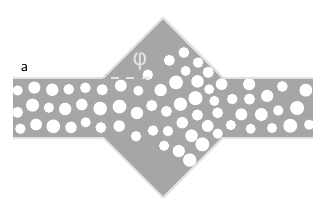
\includegraphics[width=\dimexpr\linewidth-13em\relax]{helbing_sim_example}
  \caption{Пример одной из симуляций в обсуждаемой работе}
  \label{sub:overview:helbing:sim_example}
\end{figure}

Пример одной из симуляций (с комбинацией расширения и сужения доступного пространства) можно увидеть на рисунке~\ref{sub:overview:helbing:sim_example}.


\section{Модель А. Кирчнера и А. Шадшнейдера на основе клеточного автомата}
\label{sub:overview:kirchner}

Предлагаемая авторами в работе Simulation of evacuation processes using a bionics-inspired cellular automaton model for pedestrian dynamics~\cite{kirchner2002simulation} модель представляет собой интересную вариацию модели клеточного автомата.

Краткий обзор возможностей моделей на основе клеточных автоматов можно найти в работе Cellular automata as models of complexity~\cite{wolfram1984cellular},
а более полное описание "--- в книге Cellular automata~\cite{chopard1998cellular}.

В данном же разделе представим очень краткое описание данного подхода.
Модель клеточного автомата "--- модель с дискретным пространством и определенными правилами движения по нему.
Дискретное пространство представляет собой набор клеток. Каждый пешеход занимает одну клетку.
Правила движения представляют собой набор условий, по которым пешеход переходит из своей текущей клетки в одну из соседних.

Авторы отмечают, что их разработка основывается на аналогии с биологическим процессом хемотаксиса и поведением некоторых насекомых.

Хемотаксис "--- это двигательная реакция организмов (чаще всего простейших) на химический раздражитель.
При этом химические раздражители подразделяются на аттракторы и репелленты.
Соответственно, организм движется по возрастающему градиенту аттрактора и наоборот, по убывающему градиенту репеллента.

Поведение некоторых насекомых, на которое ссылаются авторы, заключается в следующем:
каждая особь оставляет за собой некий химический след, который могут обнаружить другие особи.
В случае, если особь находит источник еды, данный химический след усиливается.
Для других особей сильный химический след является аттрактором, что приводит к определенной форме кооперации "---
набор особей более эффективно находит источники еды (по сравнению с индивидуальным поведением).

Людям свойственны намного более сложные механизмы кооперации, однако описанный механизм может служить простой моделью человеческого поведения в стрессовой ситуации,
когда сложные механизмы не используются. По мнению авторов, данный <<след>> может представлять собой некое абстрактное отображение маршрута, известного пешеходам,
а механизм накопления является аналогией следования за людьми, уже идущими по нужному маршруту.

Для реализации данной модели в рамках клеточного автомата авторы ввели два <<химических>> поля "--- статическое и динамическое.
В данном случае поле представляет собой дискретную функцию, ставящую в соответствие каждой ячейке некоторое значение.
Положительное значение представляет собой аттрактор, а отрицательное "--- репеллент.
При этом статическое поле не меняется в пределах одного запуска симуляции и представляет собой описание окружения,
где выходы являются аттракторами, а источники опасности "--- репеллентами.
Динамическое же поле используется для создания <<химического>> следа.

В рамках модели клеточного автомата в качестве правил движения было выбрано правило хемотаксиса "---
движение в строну возрастающего градиента аттрактора и наоборот, в сторону убывающего градиента репеллента.

Своей целью авторы ставят исследование различных типов поведения в стрессовых условиях.
И хотя предложенная модель на первый взгляд кажется немного странной, авторы смогли получить те же результаты,
что и другие исследователи с намного более сложными моделями (в частности, в рамках зависимости времени эвакуации от <<стадного>> поведения).
Однако в отличие от других моделей, данная модель очень проста в реализации и эффективна, что позволяет использовать ее для симуляции большего числа людей.

\begin{figure}[ht!]
  \centering
  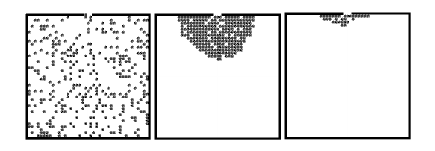
\includegraphics[width=\dimexpr\linewidth-9em\relax]{kirchner_sim_example}
  \caption{Пример одной из симуляций в обсуждаемой работе. Слева "--- изначальное положение (t = 0). Посередине "--- промежуточное положение. Справа "--- заключительная стадия (осталось всего несколько частиц)}
  \label{sub:overview:kirchner:sim_example}
\end{figure}

Пример одной из симуляций (с наблюдаемым эффектом скопления у выхода) можно увидеть на рисунке~\ref{sub:overview:kirchner:sim_example}.

\section{Агентное моделирование}
\label{sub:overview:agent}

Агентное моделирование "--- подход в моделировании сложных систем, основанный на использовании автономных <<агентов>>. Обзор данного подхода можно найти в работах
Tutorial on agent-based modelling and simulation~\cite{macal2010tutorial} и Agent-based modeling: A new approach for theory building in social psychology~\cite{smith2007agent}.
Мы же рассмотрим агентное моделирование на основе работы Agent-Based Modeling and Simulation on Emergency Evacuation~\cite{ren2009agent} за авторством Ч. Рена, Ч. Янга и С. Джина.

Данная работа предлагает следующую классификацию имитационных моделей:

\begin{itemize}
  \item имитационные модели дискретных событий;
  \item имитационные модели динамики систем;
  \item имитационные модели на основе агентов.
\end{itemize}

Имитационные модели динамики систем обычно являются макроскопическими моделями, представляющими параметры системы как некоторую функцию от времени и других параметров системы.

Имитационные модели дискретных событий обычно оперируют дискретным временем, меняя состояние системы по определенным событиям.

И наконец имитационные системы на основе агентов представляют собой микроскопические модели,
где каждый объект моделирования (<<агент>>) принимает собственные решения на основе состояния системы и параметров других агентов.
При этом правила поведения агентов должны быть достаточно простыми, а объектом исследования является то, как набор простых правил
вызывает сложные макроскопические эффекты в системе.
Как можно заметить, модель рассмотренная в разделе \ref{sub:overview:helbing} по данной классификации является имитационной моделью на основе агентов.

Далее авторы описывают свою модель на основе агентов, разработанную в среде моделирования Repast.
Данная модель концентрируется на индивидуальных параметрах классов пешеходов и их влиянии на время эвакуации.
Например, данная модель подразделяет всех участвующих пешеходов на женщин, мужчин и детей, при этом каждый класс имеет свой набор параметров.
Также в модель введены параметры <<лидерства>> и <<независимости>>, задающие соответственно желание вести других людей за собой и желание следовать за лидером.

Авторы исследуют зависимости времени эвакуации от набора параметров, таких как наличие и качество <<лидеров>> и др.
Результаты авторов совпадают с другими моделями, и может считаться их подтверждением.

Более интересным применением агентного моделирования является работа Detection of primitive collective behaviours in a crowd panic simulation based on multi-agent approach~\cite{patrix2012detection} за авторством Дж. Патрикса, А. Моуаддиба и С. Гейтпейла.

В данной работе агенты действуют в соответствии с двумя разными типами поведения, и переключаются между ними в зависимости от внешних условий.
Первый тип поведения "--- реакция (рефлекс) на некоторую рискованную ситуацию "--- возникает как непосредственный ответ на внешний стимул.
Второй тип поведения "--- сознательный "--- отвечает за долгосрочное планирование.

Так же как и авторы клеточной модели, описанной в разделе \ref{sub:overview:kirchner}, для описания коллективного поведения авторы обращаются к аналогиями из мира биологии,
в частности к тому же <<химическому>> следу феромонов муравьев и поведению стаи птиц.
Например, поведение каждой особи в стае может быть описано следующими правилами:

\begin{itemize}
  \item правило разделения: особи пытаются избежать столкновения с ближайшими особями;
  \item правило равнения: особи пытаются лететь в том же направлении, что и ближайшие особи;
  \item правило сплоченности: особи пытаются держаться недалеко от ближайших особей.
\end{itemize}

На основе всех описанных правил и типов поведения авторы строят сложную модель поведения агента.
Однако, это не является конечной целью исследования "--- авторы хотят получить возможность детектировать интересующие паттерны поведения в толпе.
Для этого авторы представили все возможные изменения внутреннего состояния агента как случайное событие, и составили цепь Маркова из этих случайных событий.
С помощью методов машинного обучения, используя последние несколько звеньев цепи Маркова, авторы пытаются детектировать определенные паттерны поведения.

Результаты данной работы включают в себя факты детектирования возникновения паники и очагов опасности, а так же успешных симуляций сложных систем.

\begin{figure}[ht!]
  \centering
  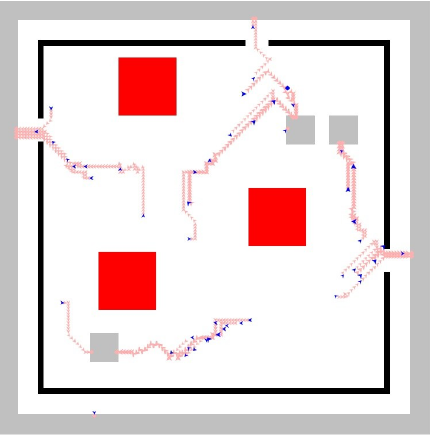
\includegraphics[width=\dimexpr\linewidth-5em\relax]{patrics_sim_example}
  \caption{Пример одной из симуляций в обсуждаемой работе. Предсказание поведения агентов в условиях паники}
  \label{sub:overview:patrics:sim_example}
\end{figure}

Пример одной из симуляций (с предсказанием поведения в условиях паники с помощью машинного обучения) можно увидеть на рисунке~\ref{sub:overview:patrics:sim_example}.


\section{Социологические и психологические исследования}
\label{sub:overview:soc}

Следует отдельно отметить множество социологических и психологический исследований паники \cite{guten1972likelihood} \cite{mawson2005understanding} \cite{quarantelli1975panic} \cite{quarantelli1999sociology} \cite{quarantelli2001sociology} \cite{quarantelli1979panic} \cite{robinette2011incorporating}.

Хотя к теме моделирования паники они явно не относятся, благодаря им и набору эмпирических наблюдений были выявлены особенности панического поведения,
которые затем могут быть применены при моделировании паники.


\section{Расчетная модель по ГОСТ 12.1.004-91}
\label{sub:overview:gost}

На территории Республики Беларусь действует ГОСТ 12.1.004-91 <<Система стандартов безопасности труда. Пожарная безопасность. Общие требования>>~\cite{gost_fire_safety},
определяющий требования пожарной безопасности к зданиям.

Также данный ГОСТ определяет требования к времени эвакуации из здания, предоставляя расчетную модель для вычисления фактического времени эвакуации.
Данная модель описана отдельно в рекомендации по расчету параметров эвакуации людей на основании положений ГОСТ 12.1.004-91 ''Пожарная безопасность. Общие требования''~\cite{model_gost}.

Расчетная модель сводится к разбиению пути эвакуации на участки, определению самого длинного (<<диктующего>>) маршрута эвакуации, и расчет времени эвакуации по этому маршруту.
Суммарное время эвакуации принимается равным сумме времени эвакуации через каждый участок.
Время эвакуации через каждый участок зависит от его расчетной длины и ширины, а также расчетного потока через этот участок.
Если поток превышает некоторый пороговый поток, то ко времени дополнительно добавляется время задержки.

Данная модель зарекомендовала себя как достаточно точный способ вычисления времени эвакуации, и может быть использована для калибровки имитационных моделей.








\section{Моделирование паники}
\label{sec:model}

В данном разделе будет дано полное описание используемой модели паники,
начиная с требований, сформулированных на основе обзора профильной литературы,
и заканчивая конкретным математическим описанием каждой из используемых социальных сил.

\subsection{Требования к разрабатываемой модели паники}
\label{sub:model:demands}

В данном разделе на основе всех вышеописанных статей и книг будут сформулированы требования к разрабатываемой модели паники.

Следует иметь ввиду, что целью данной работы является корректировка разработанной в рамках дипломного проекта имитационной модели, что накладывает определенные ограничения на требования.
В частности, итоговая модель будет представлять собой вариацию модели социальных сил, так как именно эта модель использовалась в дипломном проекте.
Будут предложены новые социальные силы, представляющие собой некоторые отображения эффектов паники, а так же изменения ядра имитационного моделирования для лучшего представления паники.

Также модель должна в той или иной степени учитывать отличия поведения людей при панике, описанные в работе Д. Хелбинга:

\begin{itemize}
  \item люди становятся более нервными, то есть быстрее и чаще принимают необоснованные решения;
  \item люди стараются двигаться значительно быстрее чем обычно;
  \item люди начинают толкаться, взаимодействия между людьми становятся физическими по природе;
  \item движение в целом и проход через узкие места в частности становятся нескоординированными;
  \item на выходах наблюдаются скопления людей;
  \item физические взаимодействия внутри толпы складываются: суммарное давление может составлять до 4500 $\text{Н} / \text{м}^2$,
        что достаточно для разрушения кирпичных стен и повреждения стальных конструкций;
  \item движение затруднено упавшими и ранеными людьми, которые становятся <<препятствиями>>;
  \item люди демонстрируют <<стадное поведение>>, то есть делают то же, что и другие люди вокруг них;
  \item люди часто не замечают запасные выходы, запасные выходы в целом используются неэффективно.
\end{itemize}

Далее будут описаны планируемые изменения модели, позволяющие учитывать названные отличия.

Для моделирования повышенного уровня нервозности хорошо подходит социальная сила флуктуаций.
Ранее, сила флуктуаций была одномоментной "--- на каждом шаге ее значение было сгенерировано случайно.
Для представления случайных необоснованных решений, данная сила будет изменена так,
чтобы флуктуации сохраняли свое направление и силу в течении некоторого периода времени.
Подробнее данное изменение будет описано в разделе \ref{sub:model:fluctuation}.

Для учета желания двигаться значительно быстрее достаточно просто увеличить желаемую скорость,
а следовательно и модуль силы притяжения к цели.

Для моделирования физических взаимодействий внесем несколько изменений в силу отталкивания.
Во-первых, значительно снизим силу отталкивания пешеходов между собой.
Во-вторых, воспользуемся предложением, описанным в работе Simulation of pedestrian crowds in normal and evacuation situations~\cite{helbing_evacuation} "---
введем увеличенную силу отталкивания при контакте и фрикционную силу, не позволяющую двигаться в тангенциальном направлении.
Подробнее данное изменение будет описано в разделе \ref{sub:model:repulsion}.

Изменения для возникновения эффекта нескоординированности прохода через узкие места, для образования скопления людей на выходе не требуются "---
данные макроскопические эффекты должны проявиться сами.

К сожалению, моделирование давления в толпе достаточно сложная тема, и потребует чрезмерного усложнения модели для своей реализации.
По этой причине, данный эффект не будет учтен в разрабатываемой модели.
Возникновение дополнительных препятствий в виде упавших и раненых людей тоже достаточно сложно реализуемо, поэтому будет опущено по той же причине.

Для <<стадного поведения>> будет введена отдельная социальная сила, копирующая направление движения ближайших соседей.
Подробнее данное изменение будет описано в разделе \ref{sub:model:herding}.

И последняя особенность (игнорирование запасных выходов) также не будет реализована в модели по причине отсутствия целеполагания
(все промежуточные точки и цели задаются еще на этапе конфигурации).
Вместо этого, данная особенность может быть учтена вручную при помощи смены целей в конфигурации сцены.

Также модель будет предлагать несколько уникальных особенностей, не учтенных в других описанных моделях.

В частности, многие модели вводят <<уровень паники>> как параметр каждого пешехода.
Этот параметр влияет на все описанные выше эффекты "--- чем выше уровень паники, тем сильнее наблюдаемый эффект.
Однако все описанные модели определяют уровень паники как константу "--- для каждого запуска симуляции уровень паники не меняется.
В реальности же паника возникает не у всех пешеходов сразу "--- она распространяется по толпе от очага возникновения.

Таким образом, в модель будет введен <<уровень паники>> для каждого пешехода,
однако он будет меняться в зависимости от уровня паники окружающих пешехода людей.
Подробнее данное изменение будет описано в разделе \ref{sub:model:panic_level}.

\subsection{Изменения в силе флуктуации}
\label{sub:model:fluctuation}

Как уже было отмечено, ранее сила флуктуации в каждый момент времени определялась как сила в случайном направлении со случайным модулем.
Для моделирования случайных иррациональных решений пешехода изменим данную силу так, чтобы она представляла некоторую случайную цель.

Определим силу флуктуации как силу, возникающую с определенной вероятностью на случайный промежуток времени,
и имеющую постоянное направление и модуль в течении этого промежутка времени.
Изначальные направление и модуль генерируются случайно в момент возникновения флуктуации.

При этом все параметры данной силы (вероятность возникновения, случайный промежуток времени действия, случайный модуль) зависят от текущего уровня паники.
Чем выше уровень паники, тем чаще флуктуации будут возникать, тем дольше они будут действовать и тем сильнее они будут.

\subsection{Изменения в силе отталкивания}
\label{sub:model:repulsion}

Напомним, что в изначальной модели сила отталкивания определялась как:

\begin{equation}
  \label{sub:model:repulstion:force_fm}
  \vec{F}_{\alpha\beta}^{repulsion}(\vec{r}_{\alpha\beta}) = - \nabla V(r_{\alpha\beta})
\end{equation}
\begin{explanation}
где & $ r_{\alpha\beta} = r_\alpha - r_\beta $ & вектор направления от $\beta$ к ближайшей точке $\alpha$; \\
    & $ V(r_{\alpha\beta}) $ & функция, эквипотенциальные линии которой имеют форму эллипса, вытянутого по направлению движения $\vec{v}_\alpha$.
\end{explanation}

Заметим, что изначальная функция отталкивания не зависела от типа препятствия.
Теперь же нам нужно иметь разную силу отталкивания от элементов конструкции (стен) и от других пешеходов.

Силу отталкивания от стен оставим без семантических изменений, лишь развернем определение функции $\nabla V$:

\begin{equation}
  \label{sub:model:repulstion:force_walls_fm}
  \vec{F}_{\alpha\beta}^{wall}(\vec{r}_{\alpha\beta}) = A exp( \frac{rad_{person} - ||\vec{r}_{\alpha\beta}||}{B} ) \frac{\vec{r}_{\alpha\beta}}{||\vec{r}_{\alpha\beta}||}
  (K + (1 - K)\frac{1 + cos(\phi_{\alpha\beta})}{2})
\end{equation}
\begin{explanation}
где & $ \vec{r}_{\alpha\beta} = r_\alpha - r_\beta $ & вектор направления от $\beta$ к ближайшей точке $\alpha$; \\
    & $ ||\vec{r}_{\alpha\beta}|| $ & дистанция от $\alpha$ до $\beta$; \\
    & $ rad_{person} $ & средний радиус пешехода; \\
    & $ A $ & коэффициент, задающий максимальную силу отталкивания; \\
    & $ B $ & коэффициент, задающий расстояние, на котором работает сила отталкивания (при $||\vec{r}_{\alpha\beta}|| = B$ сила отталкивания равна $0.36A$, при $||\vec{r}_{\alpha\beta}|| = 2B$ сила отталкивания равна $0.13A$ ); \\
    & $ \frac{\vec{r}_{\alpha\beta}}{||\vec{r}_{\alpha\beta}||} $ & нормированный вектор от $\beta$ к $\alpha$; \\
    & $ K $ & коэффициент, задающий анизотропность силы отталкивания; \\
    & $ \phi_{\alpha\beta} $ & угол между направлением движения $\vec{v}_\alpha$ и направлением к препятствию $\vec{r}_{\alpha\beta}$. \\
\end{explanation}

Базовую силу отталкивания от других пешеходов выразим аналогично силе отталкивания от стен:

\begin{equation}
  \label{sub:model:repulstion:force_pedestr_dist_fm}
  \begin{aligned}
    & \vec{F}_{\alpha\beta}^{pedestrian\ basic}(\vec{r}_{\alpha\beta}) & = A (1 - pl_\alpha) exp( \frac{2 * rad_{person} - ||\vec{r}_{\alpha\beta}||}{B} ) \\
    &                                                                             & \frac{\vec{r}_{\alpha\beta}}{||\vec{r}_{\alpha\beta}||} (K + (1 - K)\frac{1 + cos(\phi_{\alpha\beta})}{2})
  \end{aligned}
\end{equation}
\begin{explanation}
где & $ pl_\alpha $ & уровень паники пешехода $\alpha$. \\
\end{explanation}

Таким образом, при возрастании уровня паники сила отталкивания между пешеходами будет уменьшаться.

Введем новую силу отталкивания, действующую при физическом контакте:

\begin{equation}
  \label{sub:model:repulstion:force_pedestr_phys_fm}
  \vec{F}_{\alpha\beta}^{pedestrian\ phys}(\vec{r}_{\alpha\beta}) = k_{phys} (2 * rad_{person} - ||\vec{r}_{\alpha\beta}||) \frac{\vec{r}_{\alpha\beta}}{||\vec{r}_{\alpha\beta}||}
\end{equation}
\begin{explanation}
где & $ k_{phys} $ & большой коэффициент физического отталкивания. \\
\end{explanation}

И еще одну силу, препятствующую тангенциальному движению при физическом контакте:

\begin{equation}
  \label{sub:model:repulstion:force_pedestr_tangent_fm}
  \vec{F}_{\alpha\beta}^{pedestrian\ tangent}(\vec{r}_{\alpha\beta}) = k_{tangent} (2 * rad_{person} - ||\vec{r}_{\alpha\beta}||) \Delta v_{\beta\alpha}^t \vec{t}_{\alpha\beta}
\end{equation}
\begin{explanation}
где & $ k_{tangent} $ & большой коэффициент сопротивления тангенциальному движению; \\
    & $ \vec{t}_{\alpha\beta} $ & тангенциальное направление по отношению к направлению от $\beta$ к $\alpha$, получается разворотом вектора $ \frac{\vec{r}_{\alpha\beta}}{||\vec{r}_{\alpha\beta}||} $ на 90 градусов против часовой стрелки; \\
    & $ \Delta v_{\beta\alpha}^t = (\vec{v}_\beta - \vec{v}_\alpha) \vec{t}_{\alpha\beta} $ & проекция разницы скоростей $\beta$ и $\alpha$ на тангенциальное направление; \\
\end{explanation}

Итоговая сила отталкивания от пешехода определяется как:

\begin{equation}
  \label{sub:model:repulstion:force_pedestr_fm}
  \vec{F}_{\alpha\beta}^{pedestrian}(\vec{r}_{\alpha\beta}) =
    \begin{cases}
      \vec{F}_{\alpha\beta}^{pedestrian\ basic}(\vec{r}_{\alpha\beta}), & \text{если}\ ||\vec{r}_{\alpha\beta}|| > 2 * rad_{person} \\
      \vec{F}_{\alpha\beta}^{pedestrian\ phys}(\vec{r}_{\alpha\beta}) + & \\
      \vec{F}_{\alpha\beta}^{pedestrian\ tangent}(\vec{r}_{\alpha\beta}), & \text{иначе} \\
    \end{cases}
\end{equation}

А итоговая сила отталкивания как:

\begin{equation}
  \label{sub:model:repulstion:force_pedestr_fm}
  \vec{F}_\alpha^{repulsion} = \sum\limits_{\beta=walls} \vec{F}_{\alpha\beta}^{wall}(\vec{r}_{\alpha\beta}) + \\
                        \sum\limits_{\beta=pedestrians} \vec{F}_{\alpha\beta}^{pedestrian}(\vec{r}_{\alpha\beta})
\end{equation}

\subsection{Новая сила <<стадного поведения>>}
\label{sub:model:herding}

Новая сила <<стадного поведения>> призвана учесть тенденцию людей следовать за другими людьми в критических ситуациях.

Математически данную силу можно выразить как

\begin{equation}
  \label{sub:model:repulstion:force_pedestr_fm}
  \vec{F}_\alpha^{herding} = pl_\alpha \sum\limits_{\beta=pedestrians} \vec{v}_\beta
\end{equation}
\begin{explanation}
где & $ pl_\alpha $ & уровень паники пешехода $\alpha$; \\
    & $ pedestrians $ & все другие пешеходы в области видимости; \\
    & $ \vec{v}_\beta  $ & направление движения пешехода $\beta$.
\end{explanation}

Несмотря на кажущуюся простоту, можно заметить, что данная функция по своей сути рекурсивна.
Изменение направления движения одного пешехода может вызвать изменение направления движения других пешеходов,
имеющих первого пешехода в области видимости.

В общем случае, данный рекурсивный процесс может не сходится к определенному результату.
Поэтому, а так же по соображениям производительности, рекомендуется брать в качестве направления движения пешехода не текущее направление,
а направление движения на предыдущем шаге.
Таким образом рекурсия будет перенесена (<<размазана>>) во времени, не будет иметь негативных последствий для производительности,
но при этом сохранит все нужные для моделирования свойства.

\subsection{Уровень паники и его распространение}
\label{sub:model:panic_level}

В предыдущих разделах уже упоминался уровень паники каждого пешехода $pl_\alpha$.
Это число от нуля до единицы представляющее собой степень проявления эффектов паники.
Соответственно, при значении ноль эффекты паники отсутствуют, а при значении один эффекты паники проявляются сильней всего.

Как уже сообщалось ранее, большинство моделей считают уровень паники каждого пешехода константой в рамках одной симуляции.
В данном разделе будет предложена модель распространения паники.

Разрабатываемая модель предполагает наличие источников паники, а так же распространение паники среди людей в области видимости.
Источниками паники являются какие-либо опасные объекты.


Определим уровень паники на шаге $t$ как
\begin{equation}
  \label{sec:model:sf:panic:level}
  pl_\alpha^t = kspl {{1}\over{n}} \sum\limits_{i=1}^n {pl_i} + kipl {{1}\over{m}} \sum\limits_{i=1}^m {opl_i}
\end{equation}
\begin{explanation}
где & $ kspl $ & коэффициент распространения паники; \\
    & $ kipl $ & коэффициент начального приобретения паники; \\
    & $ pl_i $ & уровень паники $i$-ого пешехода; \\
    & $ opl_i $ & уровень паники $i$-ого опасного объекта; \\
    & $ n $ & количество других пешеходов в поле зрения пешехода; \\
    & $ m $ & количество опасных объектов в поле зрения пешехода; \\
\end{explanation}

Если бы мы определили итоговый уровень паники как уровень паники на шаге $t$,
то уровень паники естественно затухал бы при отдалении от опасных объектов.
В реальности же эффект паники не пропадает просто так "--- для этого нужно время.
Чтобы учесть данную закономерность, определим уровень паники на шаге $t + 1$ как:

\begin{equation}
  \label{sec:model:sf:panic:level}
  pl_\alpha^{t + 1} =
    \begin{cases}
      pl_\alpha^t, &\text{если} pl_\alpha^t > pl_\alpha \\
      kdpl (pl_\alpha - pl_\alpha^t), &\text{иначе} \\
    \end{cases}
\end{equation}
\begin{explanation}
где & $ kdpl $ & коэффициент затухания уровня паники. \\
\end{explanation}


Следует отметить важность выбора коэффициента распространения паники $kspl$ и коэффициента затухания паники $kdpl$.
Если установить для данных коэффициентов слишком низкое значение, то эффект лавинообразного возникновения паники не появится.
Если же установить слишком высокое значение, то пешеходы могут войти в состояние паники даже от незначительных воздействий.


\section{Проектирование модификаций программного средства} % (fold)
\label{sec:development}

Как уже было отмечено, данная работа представляет собой модификацию существующего программного средства, разработанного в рамках дипломного проекта.

В разделе ~\ref{sec:development:common} будет представлен общий список модификаций, выполненных в рамках работы,
и причины по которым данные модификации были необходимы.

Напомним, что программное средство состоит из трех независимых модулей:

\begin{itemize}
  \item модуль чтения и разбора схемы сооружения и сценария симуляции;
  \item модуль выполнения симуляции;
  \item модуль отображения результатов симуляции.
\end{itemize}

Модули обмениваются данными в определенном бинарном формате.

Первый модуль отвечает за разбор всей конфигурации симуляции и формирование бинарного сообщения о конфигурации второму модулю.
Данный модуль написан на языке программирования Ruby~\cite{ruby_doc}, и представляет собой имплементацию предметно"=ориентированного языка описания сценария симуляции.
Модуль не претерпевал значительных изменений в рамках разработки модификации по учету сценария массовой паники,
однако немногие изменения будут описаны в разделе~\ref{sec:development:preprocessor}.

Второй модуль является ядром программного средства, и большинство модификаций требовали изменений в этом модуле.
Написан он на языке программирования Rust~\cite{rust_doc}, и представляет собой реализацию теоретической модели пешеходных потоков.
В рамках данной работы в этот модуль была добавлена теоретическая модель поведения пешеходов в сценарии массовой паники.
Конкретные изменения будут описаны в разделе~\ref{sec:development:core}.

Последний модуль используется для отображения результатов симуляции на экране,
и написан на языке программирования C с использованием библиотеки SDL~\cite{libsdl_home}.
Список изменений, внесенных в данный модуль, можно найти в разделе~\ref{sec:development:animator}.

\subsection{Модификации программного средства}
\label{sec:development:common}

В первую очередь разрабатываемое программное средство должно реализовывать описанную в разделе~\ref{sec:model} модель паники.
Для этого необходимо внести изменения в вычисление различных социальных сил, ввести новые социальные силы,
а также добавить имплементацию модели распространения паники.
Все эти модификации касаются модуля выполнения симуляции, и будут подробно обсуждены в разделе~\ref{sec:development:core}.

Однако можно заметить, что режим работы существующего программного средства не совсем подходит для демонстрации эффектов паники.

Существующее программное средство работает в режиме <<потока>>.
На схеме сооружения существуют области появления людей (обычно располагаются на границах схемы),
генерирующие с определенной частотой новых пешеходов.
Каждый пешеход имеет набор промежуточных целей и одну конечную цель, по достижении которой он исчезает.
Таким образом генерируются непрекращающиеся <<потоки>> пешеходов от области появления до конечных целей.

И хотя данный режим позволяет оценить эффекты паники на поток пешеходов, намного более интересным является сценарий эвакуации.
В сценарии эвакуации существует определенное заранее заданное количество людей внутри сооружения.
В начале симуляции каждый пешеход находится в определенном месте, и с началом симуляции пытается добраться до выхода из здания.
Симуляция завершается, когда последний пешеход достигает своей цели.
В данном сценарии эффекты паники будут проявляться намного более наглядно, что позволит лучше их продемонстрировать.

По описанным выше причинам было решено внести в программное средство модификации,
которые позволяли бы проводить симуляцию по сценарию эвакуации
(в дальнейшем данный режим работы будем называть режимом эвакуации).
При этом важными параметрами в данном режиме являются статистические характеристики
итогового времени эвакуации для набора пешеходов, такие как минимальное и максимальное время эвакуации,
среднее время эвакуации, дисперсия времени эвакуации "---
разрабатываемое программное средство должно вычислять данные характеристики и представлять их пользователю.
Изменения, требуемые для реализации описанного режима эвакуации, были внесены во все три модуля программного средства,
и будут описаны в разделах~\ref{sec:development:preprocessor:escape}, \ref{sec:development:core:escape} и \ref{sec:development:animator}.


\subsection{Модификации модуля чтения и разбора схемы сооружения и сценария симуляции}
\label{sec:development:preprocessor}

Как уже было отмечено, модуль чтения и разбора схемы сооружения и сценария симуляции не требовал значительных модификаций.

Напомним, что сценарий симуляции имеет вид, представленный на рисунке рисунке~\ref{sec:development:preprocessor:scenario_dsl_listing}.

\begin{figure}[ht!]
  \centering
  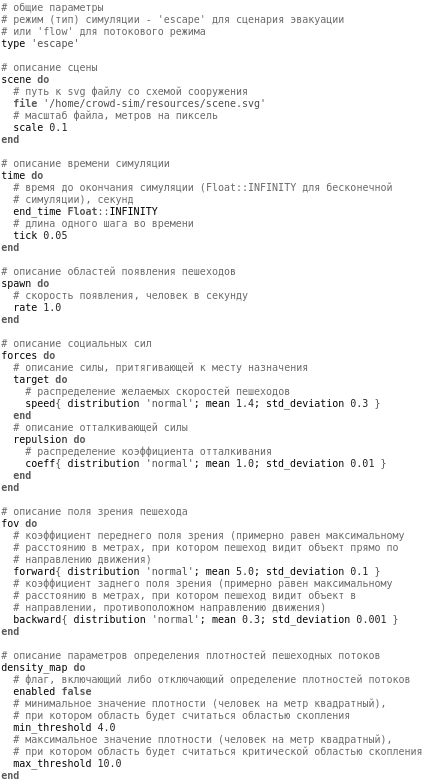
\includegraphics[width=\dimexpr\linewidth-7.0em\relax]{masters_sim_params_example}
  \caption{Пример сценария симуляции}
  \label{sec:development:preprocessor:scenario_dsl_listing}
\end{figure}

В модуль были внесены всего две модификации: поддержка различных режимов симуляции (задаются в сценарии симуляции) и поддержка источников паники (задаются в схеме сооружения).
Первая модификация описана в разделе~\ref{sec:development:preprocessor:escape}, а вторая "--- в разделе~\ref{sec:development:preprocessor:panicsource}.

\subsubsection{Режимы симуляции в сценарии симуляции}
\label{sec:development:preprocessor:escape}

В конфигурации сценария симуляции каждый параметр принадлежит определенной секции и имеет определенный номер.
Соответственно, изменение сводилось к добавлению нового параметра в секцию и присвоение ему номера.
Так как данный параметр (<<режим симуляции>>) не подходил по смыслу ни в одну существующую секцию,
для него была создана новая секция под названием <<Общие параметры>>.

Также для данного поля был введен новый тип "--- перечисление.
Данный тип позволяет указывать в сценарии симуляции строку, соответствующую набору заранее определенных строк.
При этом если строка не была найдена в заранее определенном наборе, сценарий симуляции считается неверным и выдается ошибка.
При генерировании сообщения о конфигурации элементы полей данного типа преобразуют строку в целую константу, что упрощает чтение и разбор на стороне модуля выполнения симуляции.

Таким образом, новое поле принадлежит секции <<Общие параметры>>,
и имеет тип перечисление с возможными значениями "flow" (потоковая симуляция) и
"escape" (симуляция в режиме эвакуации).

Напомним, что бинарный формат описания конфигурации (результат работы модуля, передающийся модулю выполнения симуляции)
состоит из отдельных независимых друг от друга элементов.
Каждый элемент имеет следующую структуру:
\begin{itemize}
  \item идентификатор секции, к которой принадлежит данный элемент (1 байт);
  \item идентификатор элемента внутри данной секции (2 байта);
  \item данные элемента, закодированные в бинарном формате (переменное количество байт).
\end{itemize}

Таким образом, подробно новый элемент конфигурации можно представить в виде таблицы~\ref{sec:development:preprocessor:format_table_escape}.\\[1em]

\begin{longtable}[ht]{| >{\centering}m{0.25\textwidth}
                      | >{\centering}m{0.25\textwidth}
                      | >{\centering\arraybackslash}m{0.40\textwidth}|}
\caption{Формат сообщения о конфигурации "--- режим симуляции} \label{sec:development:preprocessor:format_table_escape}\tabularnewline

\hline Секция & Элемент & Данные элемента \tabularnewline
\endfirsthead
\captionsetup{labelformat=stbtablecont,justification=raggedright}
\caption[]{}\tabularnewline
\hline 1 & 2 & 3 \tabularnewline
\endhead
  \hline Общие параметры "--- 0x00 & Режим симуляции "--- 0x0001 & \specialcell{тип (целое, 1 байт)\\
                                                                                0x01 "--- потоковая симуляция\\
                                                                                0x02 "--- симуляция сценария\\
                                                                                эвакуации}\tabularnewline
  \hline
\end{longtable}


\subsubsection{Источники паники в схеме сооружения}
\label{sec:development:preprocessor:panicsource}

В качестве схемы сооружения выступает особым образом модифицированный SVG~\cite{svg_home} файл.
SVG "--- распространенный формат векторной графики на основе XML.

Пример схемы сооружения представлен на рисунке~\ref{sec:development:preprocessor:svg_scheme_listing}.
Как видно из примера, все дополнительные параметры объектов добавлены в атрибуты с префиксом x-csim.

Для отображения источников паники была добавлена поддержка нового элемента SVG "--- circle,
атрибут x-csim-class у которого установлен в panic-source. Также у этого элемента есть дополнительный атрибут "--- x-csim-power,
задающий силу данного источника.

\begin{figure}[!htb]
  \centering
  \begin{subfigure}[!htb]{0.45\textwidth}
    \centering
    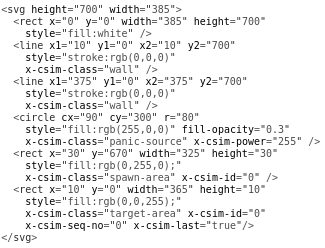
\includegraphics[scale=1.0]{masters_scene_example_text}
    \caption{}
  \end{subfigure}
  \begin{subfigure}[!htb]{0.45\textwidth}
    \centering
    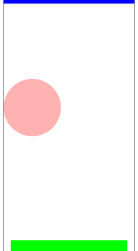
\includegraphics[scale=2.0]{masters_scene_example_pic}
    \caption{}
  \end{subfigure}
  \caption{Пример простой схемы сооружения: а "--- текстовый листинг схемы;
           б "--- схема в виде картинки}
  \label{sec:development:preprocessor:svg_scheme_listing}
\end{figure}

Описание нового элемента конфигурации, соответствующего источнику паники, можно найти в таблицe~\ref{sec:development:preprocessor:format_table_panic_source}.

\begin{longtable}[ht]{| >{\centering}m{0.25\textwidth}
                      | >{\centering}m{0.25\textwidth}
                      | >{\centering\arraybackslash}m{0.40\textwidth}|}
\caption{Формат сообщения о конфигурации "--- источник паники} \label{sec:development:preprocessor:format_table_panic_source}\tabularnewline

\hline Секция & Элемент & Данные элемента \tabularnewline
\endfirsthead
\captionsetup{labelformat=stbtablecont,justification=raggedright}
\caption[]{}\tabularnewline
\hline 1 & 2 & 3 \tabularnewline
\endhead
  \hline Сцена "--- 0x01 & Источник паники "--- 0x0004 & \specialcell{координаты центра\\
                                                                      (x, y)\\
                                                                      радиус (целое, 2 байта)\\
                                                                      сила (целое, 1 байт)}\tabularnewline
  \hline
\end{longtable}

\FloatBarrier

\subsection{Модификации модуля выполнения симуляции}
\label{sec:development:core}

Изменения, внесенные в модуль выполнения симуляции, можно разбить на несколько групп:

\begin{itemize}
  \item разбор новых параметров конфигурации;
  \item имплементация нового режима работы "--- режима эвакуации;
  \item внесение изменений в социальные силы в соответствии с моделью;
  \item добавление модели распространения паники;
  \item предоставление дополнительной информации модулю отображения результатов;
\end{itemize}

Каждая из этих групп будет описана в разделе \ref{sec:development:core:configuration},
\ref{sec:development:core:escape}, \ref{sec:development:core:forces},
\ref{sec:development:core:panic_spread}, \ref{sec:development:core:output} соответственно.


\subsubsection{Разбор новых параметров конфигурации}
\label{sec:development:core:configuration}

Разбор и сохранение конфигурации осуществляется подмодулем con\-fi\-gu\-ra\-ti\-on.
В соответствии с разделом~\ref{sec:development:preprocessor}
и таблицами~\ref{sec:development:preprocessor:format_table_escape} и~\ref{sec:development:preprocessor:format_table_panic_source},
в данном подмодуле была реализована поддержка новых параметров конфигурации.

Были добавлены функция par\-se\_ge\-ne\-ral\_item для чтения параметров из секции общих параметров,
описания необходимых структур данных для хранения новых параметров (перечисление Sim\-Ty\-pe, структура Sce\-ne\-Pa\-nicSo\-urce)
и организовано чтение новых элементов в соответствии с их идентификаторами.

\subsubsection{Режим эвакуации}
\label{sec:development:core:escape}

Как уже было описано в разделе~\ref{sec:development:common}, режим эвакуации отличается от потокового режима следующими особенностями:

\begin{itemize}
  \item создание новых пешеходов происходит один раз в начале симуляции;
  \item условием завершения симуляции является отсутствие пешеходов;
  \item необходимо выполнить подсчет статистических характеристик времени достижения цели пешеходами;
  \item данные характеристики должны быть переданы в модуль отображения результатов.
\end{itemize}

Перенос создания новых пешеходов на другой этап симуляции и замена условия завершения симуляции
тривиальны и не требуют обсуждения.

Важной задачей был подсчет статистических характеристик времени достижения цели пешеходами.
Для получения полного набора характеристик требовалось сохранить время достижения цели каждого пешехода в отдельности,
а затем проанализировать весь массив накопленных данных.

Хотя данный подход успешно работает при небольших массивах данных, в работе было принято решение использовать другой, инкрементальный подход.
Причиной принятия данного решения можно назвать устоявшуюся практику разработки программных систем, которая не поощряет
неконтролируемое разрастание операционных данных (а следовательно, и увеличение объема занимаемой оперативной памяти).
Также данное решение позволит в будущем проводить анализ больших массивов данных
(например анализ времени достижения цели в потоковой симуляции, длящейся значительный период времени).

Перейдем к описанию инкрементального подхода при расчете статистических данных.
Суть данного подхода в том, что вместо сохранения всех значений случайной величины сохраняются только ее аггрегационные параметры.
По завершению эксперимента некоторые характеристики случайной величины могут быть получены из сохраненных параметров.
Самым простым примером данного подхода является получение среднего значения путем инкрементального накопления суммы и количества элементов.

В работе также используется еще один подобный расчет для дисперсии, использующий известную формулу:

\begin{equation}
  \label{sec:development:core:escape:d_fm}
  D(X) = M(X^2) - M(X)^2
\end{equation}
\begin{explanation}
где & $ M(X) $ & математическое ожидание (среднее значение) случайной величины Х. \\
\end{explanation}

Таким образом, накапливая не только сумму значений случайно величины, но и сумму квадратов, в дальнейшем можно получить дисперсию случайно величины.

Для реализации описанного подхода был создан подмодуль sta\-ti\-stics, хранящий в себе состояние множества случайных величин.
При достижении пешеходом своей цели, подмодулю sta\-ti\-stics передается сообщение о времени достижения цели пешеходом.
В ответ на это подмодуль обновляет состояние случайной величины <<время достижения цели>>.
В состоянии сохраняются такие параметры, как минимальное и максимальное значение, сумма значений, сумма квадратов значений и количество значений.
Соответственно, по достижению конца симуляции модуль может выдать такие характеристики случайной величины, как
минимальное и максимальное значение, количество значений, среднее значение, дисперсия (и стандартное отклонение) значений.

Для передачи указанных характеристик модулю отображения результатов пришлось значительно переделать протокол взаимодействия данных двух модулей.
Подробнее об этой проблеме и путях ее решения будет рассказано в разделе~\ref{sec:development:core:output}.

\subsubsection{Изменения в социальных силах}
\label{sec:development:core:forces}

Модификации требовали две используемых социальных силы "--- сила отталкивания Re\-pul\-si\-on\-For\-ce и
сила флуктуаций Fluc\-tu\-a\-ti\-on\-For\-ce.

Изменения в силе отталкивания сводились к замене формул, используемых при расчете данной силы,
и добавлению двух новых <<отталкивающих>> сил физического контакта.

Изменения же в силе флуктуаций были более сложными в реализации.
Требовалось создать флуктуации, сохраняющиеся во времени "--- следовательно, требовалось где-то хранить такие флуктуации.
Логичнее всего казалось сохранять эти флуктуации в объекте пешехода.

Однако возникла проблема с используемой моделью заимствования языка программирования Rust.
Заимствования (получение ссылки) на объект в данном языке программирования бывают двух типов "---
с правом на модификацию и без права на модификацию.

Объекты социальных сил получали ссылки на все используемые объекты (объект пешехода и объект сцены)
без права на модификацию. Для того, чтобы изменить данный тип ссылок на ссылки с правом на модификацию,
требовались значительные изменения по всему проекту.

Чтобы избежать значительных изменений, было принято решение сохранять данные о текущих флуктуациях в самой силе флуктуации.
Для этого каждому пешеходу был назначен уникальный идентификатор, а в структуре силы флуктуации был создан ассоциативный
массив от уникального идентификатора пешехода к объекту флуктуации.
При возникновении флуктуации она сохранялась в данный ассоциативный массив и продолжала действовать до тех пор, пока ее
время действия не истекало и она не удалялась из ассоциативного массива.

Остальные изменения в силе флуктуаций также сводились к замене формул и логики расчета.

Стоит отметить, что хотя сохранение набора флуктуаций в объекте силы флуктуации сначала кажется не совсем хорошим решением
по сравнению с сохранением флуктуаций в объекте пешехода, на самом деле данное решение лучше, так как уменьшает связность
между подмодулями (правда, за счет незначительного снижения производительности "--- требуется дополнительное время на поиск
флуктуации в ассоциативном массиве по идентификатору пешехода).

Также требовалось добавить новую социальную силу <<стадного поведения>> "--- Her\-ding\-For\-ce.
Благодаря наличию аналога интерфейса в используемом языке программирования Rust, добавление новых сил в программное средство
сводится к добавлению одного модуля и регистрации его в модуле сил. Также следует отметить, что в соответствии с замечанием в
разделе~\ref{sub:model:herding} в качестве текущего вектора скорости движения берется вектор скорости движения на предыдущем
шаге.

\subsubsection{Модель распространения паники}
\label{sec:development:core:panic_spread}

Реализация модели распространения паники также было достаточно серьезным изменением.

Как уже было описано выше, потребовалось модифицировать протокол конфигурации и модуль разбора элементов конфигурации для
получения списка источников паники на схеме сооружения.
В дальнейшем данный список хранится в объекте Sce\-ne в отдельном поле для доступа и расчета параметров пешеходов.

В соответствии с моделью, в объект пешехода было добавлено поле уровня паники, имеющее тип вещественного числа от нуля до единицы.
В метод, осуществляющий обновление состояния всей модели, была добавлена логика по пересчету уровня паники для каждого пешехода
в зависимости от наличия в области видимости источника паники, от среднего значения уровня паники ближайших пешеходов и от предыдущего уровня паники.

Как и в случае с силой <<стадного поведения>>, данное моделью определение рекурсивно,
и на каждом шаге берутся значения уровня паники на предыдущем шаге.

Также для наглядной демонстрации распространения уровня паники информация о текущем уровне паники передается модулю отображения результатов.

\subsubsection{Изменения в формате протокола общения с модулем отображения результатов}
\label{sec:development:core:output}

Как было отмечено в разделе~\ref{sec:development:core:escape}, необходимо было передать модулю отображения результатов
статистические характеристики времени достижения цели пешеходов.

Проблема была в том, что главный цикл модуля отображения результатов не был рассчитан на получение различных типов сообщений.
Таким образом, модуль отображения результатов всегда ожидал сообщения одного и того же формата
(включающего в себя текущее время симуляции, положения всех пешеходов и, при наличии, параметры областей скопления).

Для решения данной проблемы были введены типы сообщений "--- каждое сообщение теперь начиналось с его типа.
Трем компонентам предыдущего формата были выделены три идентификатора типа:
0x00 для текущего времени симуляции, 0x01 для параметров всех пешеходов (положение, направление, и др.) и 0x02 для областей скоплений.
Также был добавлен четвертый тип, 0x03, для передачи статистических характеристик.

Соответствующие изменения были внесены в подмодуль out\-put "--- перед каждым сообщением посылался его тип,
и в конце симуляции посылалось одно сообщение с типом 0x03 и набором статистических характеристик.

Также изменения коснулись сообщения о параметрах всех пешеходов "--- для более наглядного отображения распространения паники,
для каждого пешехода теперь дополнительно передается его уровень паники.

\subsection{Модификации модуля отображения результатов симуляции}
\label{sec:development:animator}

Как было отмечено в предыдущем разделе, главный цикл модуля отображения результатов симуляции подвергся изменениям.
Вместо чтения целиком нового состояния симуляции, главный цикл пытается прочитать одно сообщение за раз.

В случае, если модуль получает сообщение с типом <<статистические характеристики времени достижения цели>>, симуляция считается завершенной.
После данного события модуль переходит в новый цикл, в котором генерирует текстовое представление статистических характеристик,
выводит данное текстовое представление на экран и ожидает событие ввода для завершения работы.

Текстовое сообщение генерируется с помощью библиотеки SDL\_ttf~\cite{libsdl_ttf_home}, и имеет формат
"Simulation done!\textbackslash{}nTravel time statistics: min=\%.2f, max=\%.2f, count=\%d, avg=\%.2f, variance=\%.2f, std\_deviation=\%.2f\textbackslash{}Press spacebar to exit" ,
где вместо шаблонов \%.2f и \%d подставляются реальные значения характеристик времени достижения цели.
Затем данное сообщение преобразуется в текстуру и выводится поверх экрана симуляции.  После нажатия на пробел модуль завершает работу.

Пример текстового сообщения о статистических характеристиках времени достижения цели представлен на рисунке~\ref{sec:development:animator:statistics_example}.

\begin{figure}[!ht]
  \centering
  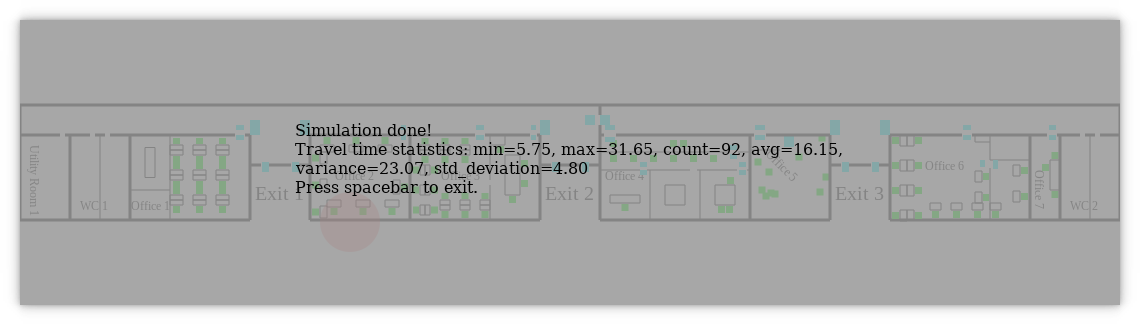
\includegraphics[width=\linewidth]{statistics_example}
  \caption{Пример отображения текстового сообщения со статистикой}
  \label{sec:development:animator:statistics_example}
\end{figure}

\begin{figure}[!ht]
  \centering
  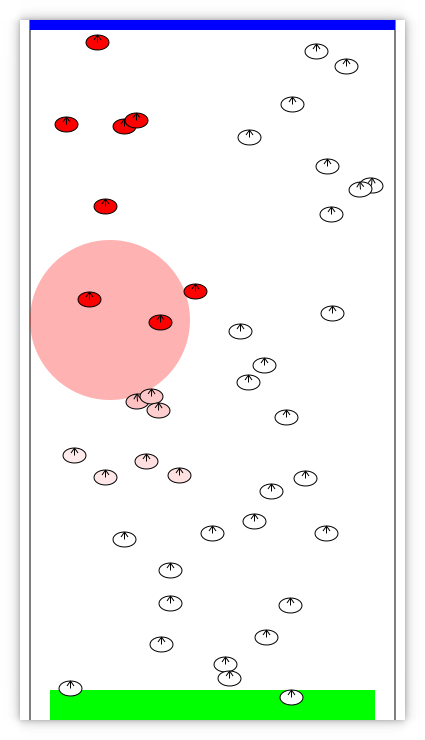
\includegraphics[scale=0.5]{panic_example}
  \caption{Пример отображения уровня паники пешеходов}
  \label{sec:development:animator:panic_example}
\end{figure}

Также модуль отображения результатов симуляции теперь отображает информацию об уровне паники каждого пешехода.
Чем выше уровень паники у конкретного пешехода, тем более его цвет смещается к красному.
Пример отображения пешеходов с высоким уровнем паники представлен на рисунке~\ref{sec:development:animator:panic_example}.

\subsection{Оценка гибкости архитектуры программного средства}
\label{sec:development:arch}

Описанные в данном разделе модификации потребовали изменения добавления около одной тысячи строк кода, и изменения еще двухсот строк кода.
Несмотря на внушительные размеры модификаций, в большинстве случаев архитектура позволяла добавлять новую логику без существенного изменения
других частей проекта.

Единственным серьезным препятствием с архитектурной точки зрения было ограничение на немутабельность (неизменяемость) сцены и пешехода в рамках расчета
социальных сил. Однако данное препятствие относительно легко решилось сменой точки зрения на требуемую функциональность.

В целом выбранную архитектуру можно считать удачной и
позволяющей без значительных проблем проводить модификацию отдельных частей программного средства.


\section{Методика использования разработанного программного средства}
\label{sec:manual}

В данном разделе будут описаны изменения в методике использования разработанного программного средства по сравнению
с методикой использования, описанной в дипломном проекте~\cite{my_diploma}.

Таким образом, данный раздел не может считаться полноценным руководством пользователя и должен
использоваться в сочетании с соответствующим разделом дипломного проекта.
Несмотря на это, для удобства раздел включает в себя все базовые понятия, необходимые для использования программного средства,
и может считаться краткой справкой по разработанному программному средству.

\subsection{Системные требования}
\label{sec:manual:requirements}

Для запуска разработанного ПС требуются следующие компоненты:
\begin{itemize}
  \item операционная система на базе GNU/Linux;
  \item установленный интерпретатор языка программирования Ruby версии 2.2 или выше;
  \item установленная библиотека SDL версии 2.0.5;
  \item установленная библиотека librsvg версии 2.40.16;
  \item установленная библиотека sdl2\_ttf версии 2.0.14;
  \item установленная библиотека librsvg версии 2.40.16.
\end{itemize}

\subsection{Входные данные симуляции}
\label{sec:manual:input}

Входными данными для симуляции являются файл сценария симуляции и файл схемы сооружения.

\subsubsection{Файл сценария симуляции}
\label{sec:manual:input:scenario}

Файл сценария симуляции использует предметно"=ориентированный язык.
Пример сценария симуляции был представлен на рисунке~\ref{sec:development:preprocessor:scenario_dsl_listing}.
% Пример сценария симуляции представлен на рисунке~\ref{sec:manual:scenario_dsl_listing}.
%
% \begin{figure}[ht!]
%   \centering
%   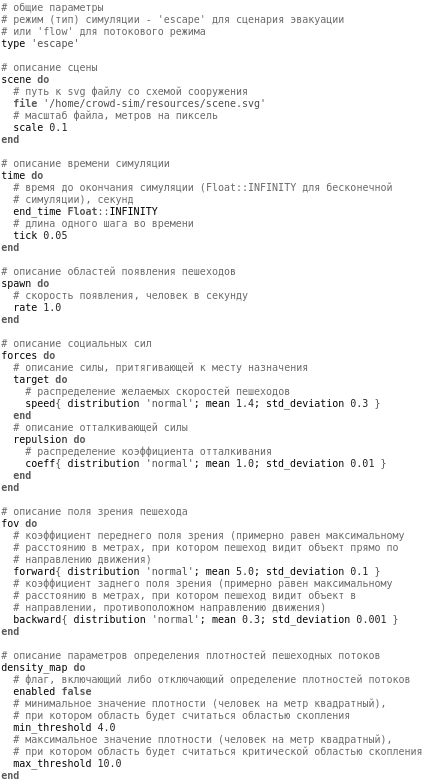
\includegraphics[width=\dimexpr\linewidth-4.5em\relax]{masters_sim_params_example}
%   \caption{Пример сценария симуляции}
%   \label{sec:manual:scenario_dsl_listing}
% \end{figure}

Описание всех полей представлено в примере сценария симуляции. Подробнее остановимся только на поле type.

Поле type задает режим симуляции и может иметь два значения.

Первое значение "--- ''flow'' "--- означает работу в режиме потока.
Блоки, помеченные как области появления людей, будут генерировать новых пешеходов в соответствии со скоростью появления,
заданной в секции spawn полем rate.
В этом режиме условием окончания симуляции является достижение времени, указанного в поле end\_time секции time.
Основное предназначение режима "--- поиск слабых мест в помещениях, где часто скапливаются пешеходы.
Чаще всего используется в сочетании с функцией по поиску мест скопления людей.
При достижении условия окончания симуляции все модули завершают свою работу без каких-либо дополнительных сообщений.

Второе значение "--- ''escape'' "--- означает работу в режиме эвакуации.
Блоки, помеченные как области появления людей, сгенерируют единственного пешехода (вне зависимости от настройки rate в секции spawn).
Условием окончания симуляции является достижение всеми пешеходами своей конечной цели.
Основным предназначением режима является определение характеристик времени эвакуации из определенного сооружения.
При достижении условия окончания симуляции модуль отображения результата выводит текстовое сообщение с
характеристиками времени эвакуации. Характеристики включают в себя минимальное и максимальное время эвакуации,
среднее время эвакуации, а также дисперсию и стандартное отклонение времен эвакуации.
Для выхода из данного состояния необходимо нажать клавишу <<пробел>>.


\subsubsection{Файл схемы сооружения}
\label{sec:manual:input:building_scheme}

Файл схемы сооружения основан на формате векторной графики SVG.
В реализованном ПС поддерживаются три элемента SVG "--- line, rect и circle.

Пример схемы сооружения представлен на рисунке~\ref{sec:manual:input:building_scheme:svg_listing}.

\begin{figure}[!ht]
  \centering
  \begin{subfigure}[!htb]{0.45\textwidth}
    \centering
    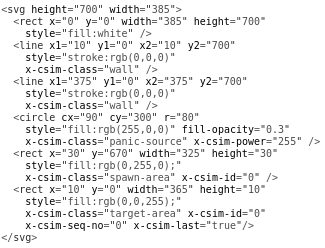
\includegraphics[scale=1.0]{masters_scene_example_text}
    \caption{}
  \end{subfigure}
  \begin{subfigure}[!htb]{0.45\textwidth}
    \centering
    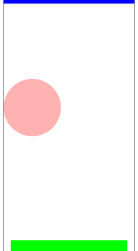
\includegraphics[scale=2.0]{masters_scene_example_pic}
    \caption{}
  \end{subfigure}
  \caption{Пример простой схемы сооружения: а "--- текстовый листинг схемы;
           б "--- схема в виде картинки}
  \label{sec:manual:input:building_scheme:svg_listing}
\end{figure}

В файле допускается использование любых элементов SVG, однако для симуляции будут иметь значение только те элементы, которым проставлен атрибут x-csim-class.
Атрибут x-csim-class отвечает за тип данного элемента.  Возможные значения данного атрибута:
  wall (препятствие),
  spawn"=area (место появления людей),
  target"=area (место назначения людей "--- промежуточное или конечное),
  panic"=source (источник паники).

Описания элементов wall, spawn"=area и target"=area было дано в дипломном проекте, остановимся на элементе panic"=source.
Для элементов с классом panic"=source должен быть проставлен атрибут x-csim-power.
Он задает силу данного источника паники, и должен иметь значение от 0 до 255
(0 "--- источник не распространяет панику, 255 "--- источник распространяет максимальный уровень паники).
Элементы класса panic"=source должны быть элементами circle, при этом желательно делать их прозрачными
(чтобы было возможность наблюдать за пешеходами и другими элементами).

\subsubsection{Запуск программного средства}
\label{sec:manual:launch}

Для запуска в режиме реального времени нужно выполнить следующую команду:
cat \$PATH\_TO\_SCENARIO \-|\- preprocessor/run.rb \-|\- \\ core/target/release/core \-|\- animator/animator animator/resources/person\_1.svg 1.0,
где \$PATH\_TO\_SCENARIO "--- путь к файлу со сценарием симуляции.


\chapter{РЕЗУЛЬТАТЫ ИСПОЛЬЗОВАНИЯ ПРОГРАММНОГО СРЕДСТВА}
\label{sec:results}

В данной главе будут описаны результаты, полученные с помощью программного средства,
основанного на разработанной модели паники.

Большинство экспериментов было поставлено в режиме эвакуации, так как данный режим
является наиболее интересным в рамках исследования моделей паники.

Для проведения экспериментов была создана схема сооружения, приближенная к реальному офисному зданию.

\begin{figure}[ht!]
  \centering
  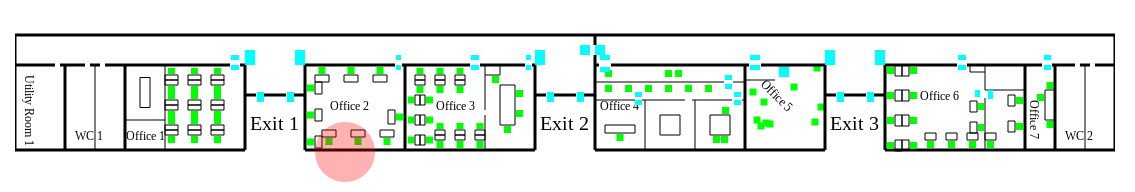
\includegraphics[width=\linewidth]{masters_office_scene}
  \caption{Схема сооружения, используемая в большинстве опытов}
  \label{sec:results:office_scene}
\end{figure}

На рисунке~\ref{sec:results:office_scene} изображена упомянутая схема сооружения.
Толстыми черными линиями обозначены стены, тонкими черными линиями "--- предметы мебели и внутриофисные перегородки.
Зеленые области соответствуют начальному положению людей в офисе.
Бирюзовые области задают промежуточные точки, которые люди должны посетить на пути к выходу.
Шесть бирюзовых областей рядом с надписями Exit 1, 2 и 3 являются конечной целью всех людей.
Розовый круг во втором офисе представляет источник паники.

\section{Влияние случайных флуктуаций на время эвакуации}
\label{sec:results:fluctuation}

Для проведения данного эксперимента была временно убрана зависимость вероятности возникновения и силы флуктуаций от уровня паники пешехода "---
уровень паники всегда считался равным 1.0, но только для силы случайных флуктуаций.

Сначала было произведено несколько контрольных замеров при силе флуктуаций равном нулю.
Время эвакуации в среднем получилось около 15 секунд, с минимумом в 5 и максимумом в 30 секунд.

При увеличении силы флуктуации до трети желаемой скорости пешехода начинают проявляться первые эффекты.
Флуктуации еще не достаточны, чтобы сбить с правильного пути пешехода, однако они уже могут значительно его замедлить.
Время эвакуации в среднем увеличивается не сильно (до 16 секунд), но максимальное время увеличивается до 40-50 секунд.

При увеличении силы флуктуации до двух третей желаемой скорости пешехода эффект становится намного более заметным.
Среднее время эвакуации увеличивается до 20 секунд, максимальное время увеличивается до 50-60 секунд.

\begin{figure}[ht!]
  \centering
  \begin{subfigure}[!htb]{0.45\textwidth}
    \centering
    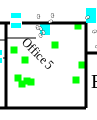
\includegraphics[scale=1.5]{masters_fluctuation_jam}
    \caption{}
  \end{subfigure}
  \begin{subfigure}[!htb]{0.45\textwidth}
    \centering
    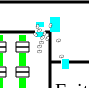
\includegraphics[scale=1.5]{masters_fluctuation_jam2}
    \caption{}
  \end{subfigure}
  \caption{Примеры пробок при большой силе флуктуации}
  \label{sec:results:fluctuation:jam}
\end{figure}

И наконец при силе флуктуации равной желаемой скорости пешехода эффект становится очень сильным.
Флуктуации достаточны, чтобы сбить пешехода с правильного пути.
Такие пешеходы сразу выбиваются из потока, пытаются идти против направления движения большинства, чем вызывают появление пробок (пример на рисунке~\ref{sec:results:fluctuation:jam}).
Среднее время эвакуации увеличивается до 40 секунд, максимальное - до 80-140 секунд.

Таким образом, случайные флуктуации (представляющие случайные иррациональные решения пешехода) оказывают строго негативное влияние на время эвакуации.
Механизм, увеличивающий время эвакуации, очевиден "--- флуктуации мешают пешеходам двигаться к своей цели кратчайшим путем,
что приводит к более длинному пути к выходу, а следовательно и к более длительной эвакуации.
При экстремальной силе флуктуаций они вызывают пробки из-за несовпадения направления движения некоторых людей в потоке с самим потоком.
Данный эффект очень сильно увеличивает время эвакуации.

\section{Влияние уменьшения силы отталкивания и использования большой силы физического контакта}
\label{sec:results:repulsion}

Как и в предыдущем разделе, воспользуемся возможностью вручную контролировать уровень паники для силы отталкивания.
Проведем эксперимент с обычной силой отталкивания (уровень паники равен нулю), а потом будем постепенно уменьшать силу отталкивания (увеличивать уровень паники)
и наблюдать за возможными эффектами.

В данном эксперименте были получены довольно интересные результаты: изменение силы отталкивания практически никак не влияет на время эвакуации.
Даже при полностью отсутствующей силе отталкивания (при использовании лишь физических сил контакта) время эвакуации не меняется.

Таким образом, выбранная модель физического контакта не способна адекватно обработать сложные физические взаимодействия.
Модели не хватает учета инерции и последствий столкновений, однако разработка такой улучшенной модели выходит за рамки данной работы.

\section{Влияние силы <<стадного поведения>>}
\label{sec:results:herding}

Проведем следующий эксперимент: будем варьировать коэффициент учета силы <<стадного поведения>> в итоговой силе, действующей на пешехода.

К сожалению, результат оказался аналогичен предыдущему разделу "---
сила <<стадного поведения>> очень слабо влияет на итоговое время эвакуации при разумном значении коэффициента.

Если выставить слишком высокое значение коэффициента, итоговое время эвакуации увеличиться, однако данный эффект имеет мало общего с реальностью.
При высоком значении коэффициента определенные пешеходы <<подхватываются>> потоком и следуют за ним некоторое время.
Однако потом такой пешеход все равно возвращается назад, так как следуя за потоком он пропустил некоторые контрольные точки на своем пути (пример на рисунке~\ref{sec:results:herding:returning}).

\begin{figure}[ht!]
  \centering
  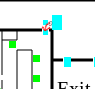
\includegraphics[scale=1.5]{masters_herding_returning}
  \caption{Примеры пешехода, возвращающегося назад после следования за потоком (стрелкой отмечено направление движения)}
  \label{sec:results:herding:returning}
\end{figure}

Таким образом, описанная проблема является не проблемой модели паники, а проблемой реализованного программного средства.
Для полноценного исследования влияния силы <<стадного поведения>> программное средство должно также реализовывать модель целеполагания пешехода.

Эффекты данной силы должны проявляться при ситуации, когда пешеход не знает текущего направления к выходу.
В таком случае данная сила должна помочь пешеходам выбрать одно направление.
Однако при слишком высоком влиянии данной силы люди могут следовать за кем-то,
кто тоже не знает направления к выходу, тем самым увеличивая время эвакуации.

Разработанное же программное средство в целях упрощения приняло, что каждый пешеход всегда знает направление к выходу.
Поэтому для исследования влияния данной силы требуется разработка модели поиска выхода для каждого пешехода, учитывающей
возможность того, что некоторые пешеходы знают направление к выходу, а некоторые "--- нет.

\section{Проявление макроскопических эффектов}
\label{sec:results:macro}

При разработке модели было высказано предположение, что некоторые макроскопические эффекты
(например, скопление людей в дверях и на выходе) должны сами проявиться при реализации простых сил модели.

Действительно, разработанная модель демонстрирует возникновение макроскопических эффектов.
Самым заметным среди них можно назвать эффект возникновения устойчивых потоков людей (рисунок~\ref{sec:results:macro:flow}).
Также возникают эффекты скопления людей в дверях (рисунок~\ref{sec:results:macro:jam}) и
нескоординированности прохода через узкие места.

\begin{figure}[ht!]
  \centering
  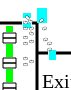
\includegraphics[scale=1.5]{masters_macro_flow}
  \caption{Пример образования устойчивого потока людей}
  \label{sec:results:macro:flow}
\end{figure}

\begin{figure}[ht!]
  \centering
  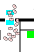
\includegraphics[scale=1.5]{masters_macro_jam}
  \caption{Пример образования скопления людей в дверях}
  \label{sec:results:macro:jam}
\end{figure}

Последний эффект очень специфичен, так как должен наблюдаться только при условии,
что через одно узкое место пешеходы пытаются пройти в разных направлениях.
В сценарии эвакуации данное условие никогда не должно наблюдаться, однако в некоторых случаях
(при очень сильной силе флуктуаций, либо иногда при неудачном стечении обстоятельств и сильном влиянии
<<стадного>> поведения) такой эффект возникает и в разрабатываемой модели.

Рисунок с примером данного эффекта уже был представлен в разделе~\ref{sec:results:fluctuation}, рисунок~\ref{sec:results:fluctuation:jam}.
В данном редком случае два пешехода пытаются пройти вправо, а два "--- влево.
В результате нескоординированности это занимает у них значительное количество времени.


\section{Модель распространения паники}
\label{sec:results:panic_spread}

В разработанном программном средстве была реализована модель распространения паники.
Для ее тестирования воспользуемся другой, более простой схемой сооружения (рисунок~\ref{sec:results:panic_spread:scene}).
На данной схеме сооружения будет единственный поток пешеходов снизу вверх. Некоторая часть этого потока попадет в зону источника паники.
При правильно подобранных коэффициентах, уровень паники во всем потоке должен возрасти до максимума.

\begin{figure}[ht!]
  \centering
  
\includegraphics[scale=0.5]{masters_panic_scene}
  \caption{Схема сооружения для тестирования паники}
  \label{sec:results:panic_spread:scene}
\end{figure}

Подбирая значения коэффициентов $k_{ipl}$, $k_{spl}$, $k_{dpl}$ добьемся вышеобозначенной цели.
На рисунке~\ref{sec:results:panic_spread:ks} представлены три этапа распространения паники:

\begin{itemize}
  \item начальный этап: первые пешеходы только получили максимальный уровень паники от источника паники;
  \item промежуточный этап: паника распространяется по пешеходам;
  \item конечный этап: все пешеходы имеют максимальный уровень паники, каждый новый пешеход также сразу получает максимальный уровень паники.
\end{itemize}

\begin{figure}[ht!]
  \centering
  \begin{subfigure}[!htb]{0.3\textwidth}
    \centering
    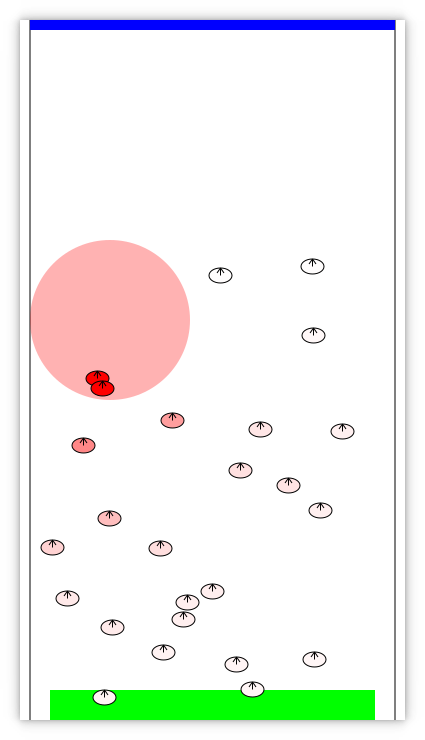
\includegraphics[scale=0.5]{masters_spread_init}
    \caption{}
  \end{subfigure}
  \begin{subfigure}[!htb]{0.3\textwidth}
    \centering
    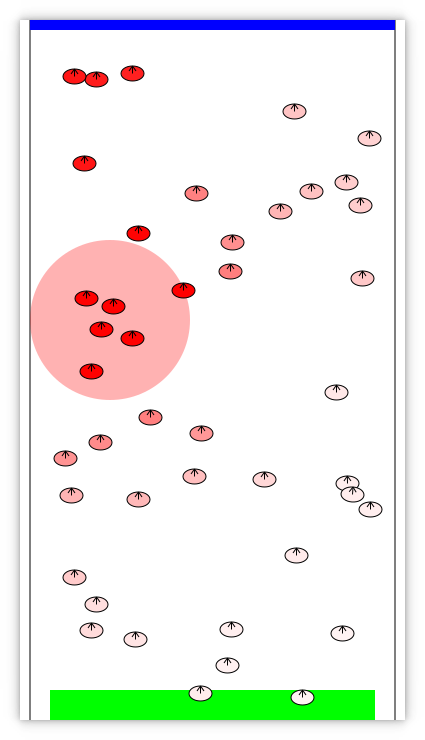
\includegraphics[scale=0.5]{masters_spread_middle}
    \caption{}
  \end{subfigure}
  \begin{subfigure}[!htb]{0.3\textwidth}
    \centering
    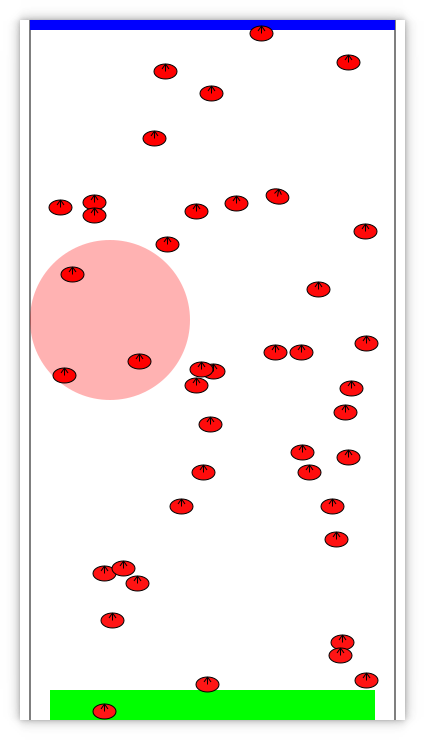
\includegraphics[scale=0.5]{masters_spread_finish}
    \caption{}
  \end{subfigure}
  \caption{Этапы распространения паники: а "--- начальный, б "--- промежуточный, в "--- конечный}
  \label{sec:results:panic_spread:ks}
\end{figure}

Такой результат был достигнут при значениях коэффициентов $k_{ipl} = 1.0$, $k_{spl} = 1.0$, $k_{dpl}$ равный утере примерно 20\% уровня паники в секунду.

Стоит отметить, что данные значения коэффициентов хорошо работают и в более сложных ситуациях, например на тестовой схеме сооружения офиса.
На рисунке \ref{sec:results:panic_spread:office} представлен пример распространения паники в офисе.

\begin{figure}[ht!]
  \centering
  \begin{subfigure}[!htb]{1.0\textwidth}
    \centering
    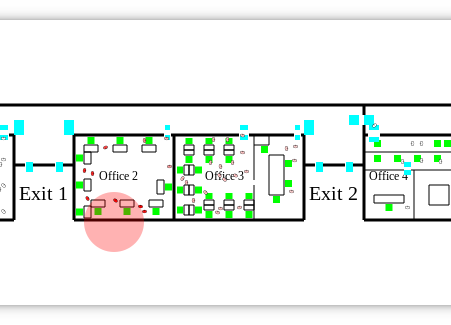
\includegraphics[width=\dimexpr\linewidth-3em\relax]{masters_spread_complex_init}
    \caption{}
  \end{subfigure}
  \begin{subfigure}[!htb]{1.0\textwidth}
    \centering
    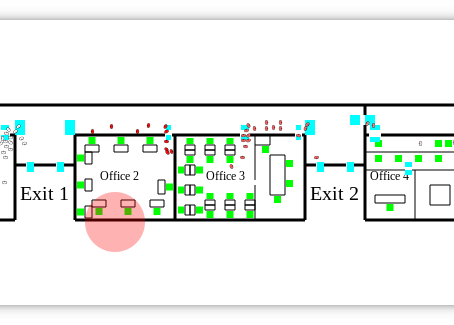
\includegraphics[width=\dimexpr\linewidth-3em\relax]{masters_spread_complex_finish}
    \caption{}
  \end{subfigure}
  \caption{Этапы распространения паники в сложной схеме сооружения: а "--- начальный, б "--- конечный}
  \label{sec:results:panic_spread:office}
\end{figure}

Можно сделать вывод, что разработанная модель распространения паники выглядит реалистично.
К сожалению, такое абстрактное понятие как <<уровень паники>> тяжело измерить,
а следовательно доказать реалистичность выбранной модели также тяжело.

\section{Влияние паники на время эвакуации с учетом всех компонентов}
\label{sec:results:general}

Проведем следующий эксперимент: установим все коэффициенты учета сил в их среднее значение
(слабо влияющее на итоговое время эвакуации), и будем варьировать наличие и количество источников паники
на схеме сооружения.

Результаты данного эксперимента совпадают с результатами эксперимента по исследованию влияния случайных флуктуаций:
при увеличении количества источников паники (либо при установке их в место, позволяющее панике распространится дальше)
среднее время эвакуации увеличивается.
Однако в данном случае время эвакуации увеличивается не так сильно "---
среднее время 16-17 секунд, максимальное - 40-50 секунд при двух источниках паники, охватывающих большинство людей.
Такие результаты получились потому что не происходит возникновения пробок из-за несогласованности прохода узких мест.

Данный эффект можно объяснить тем, что при выбранных значениях коэффициентов влияние силы <<стадного поведения>> компенсируется
влиянием силы <<стадного поведения>> "--- даже если какой-то пешеход находится под воздействием сильной флуктуации,
сила <<стадного поведения>> исправляет направление движения пешехода и заставляет двигаться вместе с потоком.

В целом, результат исследования в соответствии с разработанной моделью можно выразить в следующем:

\begin{itemize}
  \item основной причиной замедления времени эвакуации при панике является иррациональные решения пешеходов;
  \item данный эффект частично компенсируется желанием пешеходов следовать за другими пешеходами.
\end{itemize}




\chapter*{ЗАКЛЮЧЕНИЕ}
\addcontentsline{toc}{chapter}{ЗАКЛЮЧЕНИЕ}

\label{sec:final}

В рамках данной работы была разработана модель массовой паники на основе набора предложенных в научной литературе моделей
с некоторыми уникальными улучшениями.
Было также программное средство по расчету времени эвакуации с использованием разработанной модели на основе существующего
программного средства определения вероятных мест скопления людей в помещениях.

Был проведен ряд экспериментов для исследования влияния компонентов модели на время эвакуации.

Выяснилось, что некоторые компоненты модели не оказывают значительного влияния на исследуемую характеристику.
К данным компонентам можно отнести силу <<стадного поведения>> и силу физического контакта.
Причины, по которым возникла данная ситуация, разные для этих двух сил.
В случае силы <<стадного поведения>> причиной служат упрощения в выборе маршрута движения,
сделанные при разработке программного средства.
В случае силы физического контакта причиной является неполная модель движения пешеходов в общем,
и отсутствие инерции и обработки столкновений в частности.
Хотя данный результат является негативным, он указывает на определенные недостатки в модели и программном
средстве, что позволит в будущем их улучшить.

Другие компоненты модели показали лучшие результаты.
Сила случайных флуктуаций, представляющая случайные иррациональные действия пешехода,
оказывает сильно негативное воздействие на время эвакуации.
Механизм данного воздействия достаточно прост "--- сила случайных флуктуаций мешает
пешеходам двигаться к своей цели (уводит их в сторону), что приводит к более длинному пути
к цели и к более длительной эвакуации. При превышении определенного порога мощности
сила случайных флуктуаций вызывает возмущения в потоках людей, что приводит к еще большему
увеличению времени эвакуации.

Модель распространения паники также можно отнести к удачным компонентам.
К сожалению, не было найдено объективных характеристик по которым можно было бы оценить данную модель.
Однако визуально модель распространения паники показывает хорошие результаты.

При работе с разработанным программным средством также были выявлены некоторые недостатки.
Основным недостатком можно назвать отсутствие инструментария для генерации схемы сооружения.
Схема сооружения "--- файл формата SVG "--- пишется в текстовом редакторе, что занимает значительное количество времени.
Например, схема сооружения офиса используемая в исследовании была создана с помощью набора скриптов по генерации элементов
на языке программирования Ruby, и даже в таком случае ее создание заняло около 36 часов чистого времени.
Также к недостаткам программного средства можно отнести отсутствие интерактивного режима воспроизведения,
при котором можно было бы приостановить симуляцию для выполнения каких-либо действий, контролировать скорость
воспроизведения симуляции и др.

В целом, разработанный комплекс модели паники и программного средства представляет интерес для исследования,
однако пока еще не готов для применения на реальных сооружениях.
В дальнейшем работа над данным комплексом должна вестись в направлениях:

\begin{itemize}
  \item разработки редактора схем сооружения;
  \item повышения стабильности и воспроизводимости результатов;
  \item разработки интерактивного режима воспрозведения симуляции;
  \item разработки модели поиска маршрута для каждого пешехода;
  \item разработки модели движения с инерцией и столкновениями.
\end{itemize}

Каждый из этих пунктов требует значительных трудозатрат, однако при условии их выполнения программное средство потенциально
может стать очень полезным инструментом при оценке времени эвакуации из любого сооружения.



\chapter{БИБЛИОГРАФИЧЕСКИЙ СПИСОК}

\renewcommand{\bibsection}{\section*{Cписок использованных источников}}
\addcontentsline{toc}{section}{Cписок использованных источников}

\bibliographystyle{styles/belarus-specific-utf8gost780u}
\bibliography{bibliography_database}

\renewcommand{\bibsection}{\section*{Cписок публикаций соискателя}}
\addcontentsline{toc}{section}{Cписок публикаций соискателя}
\nociteown{mypub}

\makeatletter
\renewcommand\@biblabel[1]{[1"=A]}
\makeatother

\bibliographystyleown{styles/belarus-specific-utf8gost780u}
\bibliographyown{bibliography_database}


\appendix

\sectionappendix*{ПРИЛОЖЕНИЕ А\\Исходные коды разработанного программного средства}
\addcontentsline{toc}{section}{Приложение А Исходные коды разработанного программного средства}

\lstinputlisting[basicstyle=\tiny,breaklines=true]{listing.txt}


% \includepdf позволяет включить в результирующий pdf документ часть другого pdf документа, сделанного
% например не с помощью TeX. Бывает полезно, если какие-то диаграммны нарисованы, например, с помощью 
% Microoft Office и сохранены в pdf.
%\includepdf[pages={-}]{documents_list.pdf}

\end{document}
